\documentclass[conference]{IEEEtran}
\usepackage[T1]{fontenc}
\usepackage[utf8]{inputenc}
\usepackage{hyperref}
\usepackage{times}
\usepackage{microtype}
\usepackage{xurl}
\usepackage{graphicx}
\usepackage{amsmath}
\usepackage{amssymb}
\Urlmuskip=0mu plus 2mu\relax
\usepackage{enumitem}

\title{\textbf{Energy-Aware V2X Handoff Under Adverse Propagation:\\ A Weather- and Interference-Aware Simulation Study}}
\author{Ranesh Das Rik \\ Department of ETE \\ RUET}
\setlist[itemize]{leftmargin=*,topsep=2pt,itemsep=1pt,parsep=0pt,partopsep=0pt}

\begin{document}
\raggedbottom
\maketitle
\emergencystretch=4em

\section{Proposed paper / conference titles}
\begin{itemize}
\item \textbf{Energy-Aware V2X Handoff Under Adverse Propagation: A Weather- and Interference-Aware Simulation Study}
\item \textbf{Green V2X Mobility Management: Energy-Per-Bit Guided Handoff With QoS and Stability Constraints}
\item \textbf{Beyond RSSI: Cross-Layer Energy-Aware Handoff for Sustainable V2X Communications}
\item \textbf{Reducing Communication Energy and CO2 in V2X Networks via Load-Aware Energy-Optimal Handoff}
\item \textbf{Robust Energy-Aware Handoff for V2X: Sensitivity, Scalability, and Scenario-Diversity Evaluation}
\item \textbf{Service-Preserving Energy Minimization in Vehicular Handoffs Using EPB-Based Association}
\item \textbf{A Multi-Baseline Benchmark of Energy-Aware Handoff in V2X Networks}
\item \textbf{Interference- and Weather-Aware Handoff Optimization for Energy-Efficient V2X Connectivity}
\item \textbf{Toward Carbon-Efficient V2X Networking: An Energy-Aware Handoff Framework and Evaluation}
\item \textbf{Stability-Constrained Energy-Aware Handoff for V2X: Hysteresis, TTT, and Cooldown in Practice}
\item \textbf{From RSSI to Sustainability: Energy and Emission Impacts of Handoff Policy Design in V2X}
\item \textbf{Scalable Green Handoff Control for Vehicular Networks: An Energy and CO2 Perspective}
\end{itemize}


\section{Abstract}

Wireless communication for intelligent transport contributes to ICT electricity use and, through grid power, to operational CO\textsubscript{2} emissions. This work studies how \textbf{mobility management (handoff)} affects the \textbf{communication energy} and \textbf{grid-electricity carbon footprint} of vehicular V2X links---without claiming to model vehicle propulsion, manufacturing, or backbone transport networks. Vehicular networks rely on handoff to keep fast-moving users connected; conventional triggers (RSSI/SINR-centric) can select high-power links, concentrate load on busy base stations, and induce ping-pong under fading---raising energy-per-bit (EPB) and, when Joules are mapped to kg CO\textsubscript{2} using a \textbf{configurable grid emission factor}, operational emissions.

This project presents a research-grade, reproducible V2X simulator and an \textbf{energy-aware handoff} policy that minimizes EPB with a load penalty while preserving QoS and stability. The simulator uses weather-dependent propagation, interference-aware SINR, Shannon-style achievable rates, and a TX-chain energy model (PA efficiency, circuits, baseband, cooling) whose parameter ranges are consistent with classical cellular energy studies \cite{auer2011howmuch,hasan2011green}. Carbon metrics use \textbf{operational radio-access communication energy} only; an optional extended breakdown (infrastructure-style overhead, optional amortized embodied base-station carbon) is available in code for scope discussion but is not the default headline metric.

\textbf{Scope (CO\textsubscript{2}):} We quantify \textbf{operational RF communication energy} and its \textbf{grid CO\textsubscript{2}} proxy; \textbf{vehicle propulsion, OBU/RSU manufacturing, backhaul transport, and non-radio subsystems are out of scope.} The default grid intensity (e.g.\ 0.5~kg~CO\textsubscript{2}/kWh) is a global-style average; for regional policy relevance, results can be re-run with a \textbf{Bangladesh-oriented factor} (order 0.6--0.65~kg~CO\textsubscript{2}/kWh per national grid reporting). \textbf{Yearly per-vehicle CO\textsubscript{2}} from short runs uses linear scaling and should be read as an \textbf{illustrative upper bound under continuous full-rate operation} unless multiplied by a \textbf{duty cycle} (e.g., 10\%, 25\%, 50\%) reflecting real usage---see the duty-cycle discussion in this note.

The energy-aware policy ranks base stations by EPB$\times$(load penalty), with QoS filters, hysteresis, time-to-trigger, cooldown, and ping-pong control. Benchmarks include RSSI, SINR, load-aware RSSI, and naive nearest baselines under fair PHY. The evaluation reports energy, EPB, CO\textsubscript{2}, handoffs, throughput, outage, and availability across multiple seeds (paired tests), plus scalability, energy-model sensitivity, scenario diversity, and optional \textbf{validation} utilities (literature EPB anchors, multi-duration rate stability). Together, the results support energy-aware handoff as a tool for reducing \textbf{communication-side} energy and emissions in V2X studies, with explicit limitations for sustainability-oriented venues.


\section{Overview: What this project is about}

\paragraph*{Framing (energy and environment)}
The ICT sector accounts for a few percent of global electricity use \cite{malmodin2018global}; vehicular connectivity adds load at the radio access edge. This project treats \textbf{sustainable V2X} as: reduce \textbf{communication energy} and \textbf{grid-CO\textsubscript{2} proxies} from handoff policy under explicit \textbf{scope} (Section ``CO\textsubscript{2} and grid accounting''). For developing-region venues (e.g.\ Bangladesh), reporting a \textbf{regionally plausible grid intensity} alongside a global default strengthens policy relevance.

\paragraph*{High-level idea}
\begin{itemize}
\item \textbf{Goal}: This project builds a \textbf{vehicular V2X network simulator} to compare traditional handoff algorithms (like RSSI-based) against a new \textbf{energy-aware handoff} policy.
\item \textbf{Core claim}: You can \textbf{reduce energy-per-bit and CO\textsubscript{2} (communication-side)} in vehicular networks \textbf{without breaking QoS} (throughput, outage, availability) by:
\item Making handoff decisions based on \textbf{energy per delivered bit (EPB)},
\item Adding a \textbf{load penalty} (avoid overloaded BSs),
\item And using \textbf{hysteresis + time-to-trigger + ping-pong control} to prevent flapping.
\end{itemize}

When you run \texttt{python main.py}, it:
\begin{itemize}
\item Creates a \textbf{sparse, high-fading vehicular scenario} (highway-like).
\item Runs \textbf{5 random seeds}.
\item For each seed runs \textbf{5 algorithms}:
\item Energy-aware, RSSI, SINR, load-aware RSSI, naive nearest.
\item Computes \textbf{detailed metrics} (energy, CO2, EPB, throughput, outage, availability).
\item Saves:
\item \textbf{Plots} (energy, CO2, distributions, topology).
\item \textbf{JSON} results for reproducible, “paper-style” analysis.
\item Then runs \textbf{three experiment families}:
\item \textbf{Scalability} vs number of vehicles.
\item \textbf{Energy-model sensitivity} (change power model parameters).
\item \textbf{Scenario diversity} (clear / heavy rain / urban dense).
\item Optional: \textbf{Comprehensive validation} (\texttt{python main.py --comprehensive-validation} or \texttt{python validation\_runner.py}): literature EPB checks, multi-duration extrapolation stability, extended CO\textsubscript{2} example, literature index printout.
\end{itemize}


\section{CO\textsubscript{2} and grid accounting (scope for energy conferences)}
\label{sec:co2_scope}

\paragraph*{What is included}
\begin{itemize}
\item \textbf{Operational communication energy} of the vehicular uplink chain as modeled (TX power control, Shannon rate, EPB, handoff overhead).
\item \textbf{CO\textsubscript{2}} as Joules $\rightarrow$ kWh $\times$ \textbf{carbon intensity} kg CO\textsubscript{2}/kWh (\texttt{SimulationConfig.carbon\_intensity\_kg\_per\_kwh}).
\item Optional in code: \texttt{ComprehensiveEnvironmentalMetrics} adds labeled breakdown (direct comms; optional infrastructure overhead factors; optional amortized embodied BS carbon) and \texttt{co2\_scope\_statement} text in simulator stats.
\end{itemize}

\paragraph*{What is excluded (must appear in the camera-ready paper)}
\begin{itemize}
\item Vehicle \textbf{propulsion} energy and tailpipe emissions.
\item \textbf{Manufacturing} and disposal of vehicles, OBUs, and infrastructure.
\item \textbf{Backhaul} and core network transport energy.
\item End-user devices other than the modeled vehicular radio chain.
\end{itemize}

\paragraph*{Bangladesh / regional grid intensity}
The codebase default is \textbf{0.5}~kg~CO\textsubscript{2}/kWh (global-average-style). For Bangladesh-focused discussion, re-run with \textbf{0.62}~kg~CO\textsubscript{2}/kWh (illustrative; align with Power Development Board / national emission-factor publications when you cite). Report both if you compare global vs local policy narratives.

\paragraph*{Yearly CO\textsubscript{2} and duty cycle}
The metric \texttt{co2\_kg\_per\_vehicle\_per\_year} linearly scales simulated fleet CO\textsubscript{2} by $\tau_y/\tau_{\mathrm{sim}}$ assuming the simulated interval is representative of the \textbf{same duty cycle} over the year. Short runs (e.g.\ 800~s) are useful for \textbf{relative} algorithm comparison; \textbf{absolute} annual figures should be labeled as \textbf{illustrative} or multiplied by a \textbf{duty cycle} $\delta\in(0,1]$ (radio active fraction of the year):

\begin{center}
\begin{tabular}{|c|c|}
\hline
\textbf{Duty cycle $\delta$} & \textbf{Interpretation} \\
\hline
1.0 & Upper bound: continuous full-rate operation over the year \\
\hline
0.5 & Radio active half of the time (example) \\
\hline
0.25 / 0.10 & More conservative usage assumptions \\
\hline
\end{tabular}
\end{center}

\noindent\textbf{Scaled annual CO\textsubscript{2}} $\approx \delta \times$ \texttt{co2\_kg\_per\_vehicle\_per\_year} (same linear scaling assumption).


\section{Project architecture: main components}

\subsection{1. Entry point: \texttt{main.py}}

\paragraph*{What it does}
\begin{itemize}
\item Sets \textbf{global experiment parameters} (seeds, vehicle counts for scaling, energy model sweep values, etc.).
\item Builds a \textbf{default configuration}: \texttt{SimulationConfig.sparse\_demonstration\_scenario()}.
\item For each seed:
\item Updates \texttt{config.seed}.
\item Creates a \texttt{V2XSimulator}.
\item Calls \texttt{simulator.run\_comparison()} → runs all algorithms and comparison.
\item Aggregates \textbf{per-seed statistics} and prints \textbf{multi-seed mean ± std}.
\item Runs \textbf{paired t-tests} comparing energy-aware vs RSSI (on total energy and average EPB).
\item Converts energy into \textbf{CO2} using grid carbon intensity.
\item Saves the last seed’s full results (\texttt{results/simulation\_results.json}).
\item Uses \texttt{ResultVisualizer} to create \textbf{all plots}.
\item Launches three experiment helpers:
\item \texttt{run\_scaling\_experiment}
\item \texttt{run\_energy\_model\_sensitivity}
\item \texttt{run\_scenario\_diversity\_experiment}
\item Optional CLI: \texttt{python main.py --comprehensive-validation} (or \texttt{python validation\_runner.py}) for literature EPB validation, multi-duration extrapolation checks, and CO\textsubscript{2} scope example output.
\end{itemize}

So \texttt{main.py} is the “orchestrator” that:
\begin{itemize}
\item Configures a base scenario.
\item Drives all algorithms and experiments.
\item Summarizes results in console + \texttt{results/} folder.
\end{itemize}


\subsection{2. Simulator core: \texttt{V2XSimulator} (\texttt{simulations/simulator.py})}

\paragraph*{Responsibilities}
\begin{itemize}
\item Represents an entire V2X system for a given configuration \texttt{SimulationConfig}.
\item Owns:
\item List of \texttt{BaseStation} objects.
\item List of \texttt{Vehicle} objects.
\item One shared \texttt{EnergyModel} (optional literature calibration via \texttt{use\_energy\_calibration} in \texttt{SimulationConfig}).
\item \texttt{EnvironmentalMetrics} for J $\rightarrow$ kg CO\textsubscript{2} (primary reporting).
\item \texttt{ComprehensiveEnvironmentalMetrics} for optional extended CO\textsubscript{2} breakdown and scope strings in stats.
\item Algorithm instances:
\item \texttt{EnergyAwareHandoff}
\item \texttt{RSSIHandoff}
\item \texttt{SINRHandoff}
\item \texttt{LoadAwareRSSIHandoff}
\item \texttt{NaiveNearestHandoff}
\item Exposes main methods:
\item \texttt{setup\_network()}
\item \texttt{setup\_vehicles()}
\item \texttt{run\_algorithm(algorithm\_name)}
\item \texttt{run\_comparison()}
\item \texttt{save\_results(filename)}
\end{itemize}



\section{System / scenario modeling}

\subsection{1. Network topology: \texttt{setup_network}}
\begin{itemize}
\item Creates a \textbf{grid of base stations} inside a square of side \texttt{area\_size}.
\item \texttt{num\_base\_stations} is assumed to be a perfect square or near-square:
\item \texttt{grid\_size = sqrt(num\_base\_stations)}
\item BSs placed on a grid with spacing \texttt{spacing = area\_size // (grid\_size + 1)}.
\item Each BS gets a \texttt{BSConfig} with:
\item \texttt{coverage\_radius} (disc of coverage).
\item \texttt{shadowing\_std\_db} (from the \textbf{weather profile}).
\item \texttt{path\_loss\_exponent} (also from weather).
\item \texttt{rain\_attenuation\_db\_per\_km}.
\item \texttt{target\_rx\_power\_dbm} (target at receiver).
\item \texttt{shadowing\_reliability} (percentile margin for coverage).
\item This uses \texttt{SimulationConfig.get\_weather()} which gives scenario-dependent:
\item Path loss exponent,
\item Shadowing standard deviation,
\item Rain attenuation.
\end{itemize}

\textbf{Result}: a grid of BSs with realistic channel parameters (path loss, shadowing, rain).


\subsection{2. Vehicle mobility: \texttt{setup_vehicles}}
\begin{itemize}
\item For each \texttt{vehicle\_id} in \texttt{0..num\_vehicles-1}:
\item Sample a \textbf{speed} between \texttt{vehicle\_speed\_min} and \texttt{vehicle\_speed\_max}.
\item If \texttt{movement\_mode == "highway"}:
\item Compute lane centerlines via \texttt{highway\_lane\_centers\_y()}.
\item Each vehicle is assigned a lane index \texttt{lane\_idx = i \% num\_lanes}.
\item For that lane:
\item Lane-specific speed bounds via \texttt{highway\_lane\_speed\_bounds(lane\_idx)}; higher lanes can have higher speeds.
\item Sample lane speed in that range.
\item Set starting \texttt{x} uniformly in \texttt{[0, area\_size]} and \texttt{y} equal to lane center.
\item Direction set to \texttt{highway\_direction\_rad} (straight line).
\item Vehicles have lane metadata (lane index, lane y).
\item Else (non-highway):
\item Sample \texttt{(x, y)} uniformly on the area.
\item Sample direction uniformly in \texttt{[0, 2π)}.
\end{itemize}

\paragraph*{Highway dynamics}
\begin{itemize}
\item \texttt{\_maybe\_highway\_lane\_switch(vehicle, current\_time)}:
\item Only active when \texttt{movement\_mode == "highway"}.
\item Uses:
\item \texttt{highway\_lane\_switch\_prob\_per\_s} to compute per-step probability.
\item \texttt{highway\_lane\_switch\_cooldown\_s} to enforce a cool-down.
\item If triggered:
\item Vehicle moves to an adjacent lane (index ±1).
\item \texttt{y} is updated to new lane center.
\item Speed is resampled from that lane’s speed bounds.
\item \texttt{Vehicle.move()}:
\item Moves the vehicle by \texttt{speed * delta\_time} along direction.
\item Wraps at borders (for straight highway).
\item Optionally adds \textbf{lateral Gaussian noise} (\texttt{highway\_lateral\_noise\_std\_m}) to simulate slight wandering within the lane.
\end{itemize}

\textbf{Result}: vehicles follow highway-like trajectories with rare lane changes and lane-dependent speed.



\section{Channel, link, and energy modeling}

\subsection{1. Per-step link metrics: \texttt{_make_step_link_metrics_getter}}

This is a critical part: it builds a function \texttt{get\_link\_metrics(vehicle, bs, require\_capacity)} that is used by \textbf{all} algorithms in a time step.

It handles:
\begin{itemize}
\item \textbf{Coverage check}: if vehicle not in BS coverage disc → \texttt{None}.
\item Possible \textbf{capacity limit} (if implemented in \texttt{BaseStation.has\_capacity()}).
\item \textbf{Shadowing}:
\item For each pair \texttt{(bs\_id, vehicle\_id)}, draw one shadowing sample and \textbf{cache it}.
\item Reused for:
\item Algorithm decision,
\item Energy metrics,
\item SINR calculation.
\item This avoids “randomness changing when you call it more times”.
\item \textbf{Distance} and \textbf{required TX power}:
\item \texttt{distance = bs.distance\_to(x, y)}
\item \texttt{tx\_power = bs.calculate\_tx\_power\_required\_for\_target\_rx(distance)}
\item Convert to dBm, apply path loss and shadowing to compute \texttt{rx\_power}.
\item \textbf{Interference and SINR}:
\item For the same vehicle:
\item Loop over \textbf{all other BSs}.
\item For each other BS, compute its signal at this vehicle (with its own shadowing sample).
\item Sum them as \texttt{interference\_mw}.
\item Thermal noise:
\item \texttt{noise\_dbm = -174 dBm/Hz + 10 log10(20 MHz)}.
\item Convert to linear \texttt{noise\_mw}.
\item \texttt{sinr\_linear = signal\_mw / (interference\_mw + noise\_mw)}.
\item \texttt{snr} in dB (here effectively SINR).
\item \textbf{Data rate \& energy per bit}:
\item If \texttt{snr <= snr\_outage\_threshold\_db}:
\item Outage: \texttt{data\_rate = 0}, \texttt{energy\_per\_bit = ∞}.
\item Else:
\item Shannon formula: \texttt{data\_rate = max(1e5, 20e6 * log2(1 + 10^(snr/10)))}.
\item EPB via \texttt{EnergyModel.calculate\_energy\_per\_bit(tx\_power, data\_rate, packet\_size)}.
\end{itemize}

It returns a dict with:
\begin{itemize}
\item \texttt{distance}, \texttt{tx\_power}, \texttt{rx\_power}, \texttt{snr} (dB), \texttt{interference\_mw}, \texttt{data\_rate}, \texttt{energy\_per\_bit},
\item plus:
\item \texttt{bs} itself,
\item \texttt{load} from \texttt{bs.get\_load()},
\item \texttt{metric = energy\_per\_bit * (1 + 2 * load)} which is the \textbf{energy+load metric} used by the energy-aware policy.
\end{itemize}


\subsection{2. Energy model \& CO\textsubscript{2}}
\begin{itemize}
\item \texttt{EnergyModel} (\texttt{src/models/energy.py}):
\item Models \textbf{total TX-chain power} for vehicle transmit (default \texttt{device\_type='obu'}):
\item \( P_\text{total} = \frac{P_\text{tx}}{\eta_\text{pa}} + P_\text{tx\_circuit} + P_\text{baseband} + P_\text{cooling} \)
\item Parameter choices (e.g.\ PA efficiency, circuit power) should be justified against ranges discussed in cellular energy literature \cite{auer2011howmuch,hasan2011green}; optional OBU-scale calibration can align EPB with literature anchors (\texttt{src/utils/hardware\_validation.py}, \texttt{representative\_model\_epb\_predictions}).
\item \texttt{calculate\_total\_power(tx\_power, 'transmit', device\_type)} and \texttt{calculate\_energy\_per\_bit(..., device\_type)}.
\item Shannon-capacity style rate plus EPB is a standard simulation methodology for green wireless studies \cite{chen2011fundamental}.
\item \texttt{EnvironmentalMetrics}:
\item Parameter: \texttt{carbon\_intensity\_kg\_per\_kwh} (default 0.5; set \textbf{0.62} for Bangladesh-style sensitivity runs).
\item \texttt{energy\_to\_co2(E) = (E / 3.6e6) * carbon\_intensity\_kg\_per\_kwh}.
\item \texttt{avg\_co2\_kg\_per\_vehicle}, \texttt{co2\_kg\_per\_vehicle\_per\_year} (see duty-cycle caveat above).
\item \texttt{ComprehensiveEnvironmentalMetrics}: optional infrastructure/embodied terms; stats expose \texttt{co2\_breakdown\_comprehensive}, \texttt{co2\_scope\_statement}.
\end{itemize}

\paragraph*{Handoff energy}
\begin{itemize}
\item Every time \texttt{\_execute\_handoff} is called:
\item Add a fixed \texttt{handoff\_energy\_joules}.
\item Add extra transmit energy during handoff delay:
\item Compute \texttt{tx\_power} to new BS.
\item Multiply \texttt{EnergyModel.calculate\_total\_power(tx\_power, 'transmit', device\_type='obu')} × \texttt{handoff\_delay\_s}.
\item Update \texttt{last\_handoff\_time}.
\end{itemize}



\section{The algorithms: how each policy works conceptually}

All algorithms implement:
\begin{itemize}
\item \texttt{select\_best\_bs(...)} → propose candidate BS (and info).
\item \texttt{should\_handoff(...)} → apply decision rule.
\item \texttt{execute\_handoff(...)} → change serving BS and update algorithm statistics.
\end{itemize}


\subsection{1. Energy-Aware Handoff (core algorithm)}

\paragraph*{Objective}
\begin{itemize}
\item Minimize \textbf{energy per delivered bit}, while:
\item Avoiding overloaded BSs (load penalty),
\item Maintaining QoS (min data rate, outage threshold),
\item Limiting unnecessary handoffs (hysteresis, time-to-trigger, cooldown, ping-pong window).
\end{itemize}

\paragraph*{Key elements}
\begin{itemize}
\item \textbf{Per-link metric}:
\item From \texttt{get\_link\_metrics}: \texttt{metric = energy\_per\_bit * (1 + 2 * load)}.
\item \textbf{QoS filter}:
\item Only consider BSs whose \texttt{data\_rate >= min\_data\_rate\_bps} and \texttt{snr > snr\_outage\_threshold\_db}.
\item If none meet QoS, falls back to best energy among those available (tests verify fallback).
\item \textbf{Decision rule} (\texttt{should\_handoff}):
\item Compute:
\item \texttt{current\_epb} for current BS.
\item \texttt{candidate\_epb} for best candidate.
\item Only handoff if:
\item \texttt{candidate} offers at least \texttt{energy\_aware\_min\_energy\_saving} relative saving (hysteresis in EPB).
\item Enough time has passed since last handoff (\texttt{handoff\_cooldown\_s}).
\item The saving persists or is statistically meaningful (time-to-trigger semantics).
\item \textbf{Ping-pong protection}:
\item \texttt{ping\_pong\_window\_s}:
\item Track last handoff event \texttt{(time, from\_bs, to\_bs)} per vehicle.
\item If within window a reversal \texttt{A→B} then \texttt{B→A} occurs, it’s counted as ping-pong and discouraged.
\end{itemize}

\paragraph*{Effect}
\begin{itemize}
\item Tends to:
\item \textbf{Avoid very high TX power} links.
\item Prefer links with \textbf{good SINR} and moderate TX power.
\item Avoid \textbf{overloaded BSs} by penalizing load in metric.
\item In results:
\item Lower average EPB,
\item Often lower TX power distribution median,
\item More balanced BS loads,
\item Similar or slightly better SINR distribution in low-percentile region.
\end{itemize}


\subsection{2. RSSI-based handoff}

\paragraph*{Baseline}
\begin{itemize}
\item Classic approach:
\item Pick BS with \textbf{strongest received signal strength} (RSSI).
\item In this simulator:
\item Still uses \textbf{adaptive TX power} to reach a target RX level (PHY-fair baseline).
\item Decision rule:
\item At each step:
\item Use link metrics to get \texttt{rx\_power} for current and candidate BS.
\item Handoff if candidate’s RSSI is higher under some policy (e.g., no or small hysteresis).
\end{itemize}

\paragraph*{Note on fairness}
\begin{itemize}
\item By \textbf{adaptively choosing TX power} for RSSI baseline (instead of fixed TX), you avoid giving energy-aware an unfair advantage just from “using power control” while baseline doesn’t.
\item There is a \textbf{fixed-TX sensitivity mode} for RSSI (\texttt{rssi\_energy\_use\_fixed\_tx}) that:
\item Keeps the algorithm’s PHY the same (adaptive),
\item But separately computes “what if TX was fixed” for energy sensitivity analysis.
\end{itemize}


\subsection{3. SINR-based handoff}
\begin{itemize}
\item Similar structure but uses \textbf{instantaneous SINR} instead of RSSI:
\item Select BS with highest SINR.
\item Handoff if candidate SINR is better according to \texttt{should\_handoff}.
\item For energy comparison:
\item To be consistent, the simulator uses the \textbf{energy-aware EPB calculation} to estimate EPB if vehicle attached to the SINR-selected BS.
\end{itemize}


\subsection{4. Load-aware RSSI}
\begin{itemize}
\item Hybrid:
\item Handoff metric = \texttt{rx\_power - α * load}, with \texttt{α = load\_penalty\_alpha\_db}.
\item So high RSSI but overloaded BS might be less attractive.
\end{itemize}


\subsection{5. Naive nearest BS}
\begin{itemize}
\item Geometry-only:
\item Select BS with \textbf{minimum Euclidean distance}.
\item Ignores:
\item Shadowing,
\item Interference,
\item Path-loss exponent beyond distance.
\item Energy and QoS metrics still computed with full model; only the decision logic is naive.
\end{itemize}



\section{Simulation loop: how a full run of an algorithm works}

Inside \texttt{run\_algorithm(algorithm\_name)}:
\begin{itemize}
\item \textbf{Reset state}:
\item For each vehicle:
\item \texttt{reset\_stats()} (energy, bits, handoffs, etc.).
\item For each base station:
\item Clear \texttt{connected\_vehicles}.
\item \textbf{Select appropriate algorithm object}.
\item \textbf{Initial association (t=0)}:
\item Build an initial \texttt{get\_link\_metrics} function.
\item For each vehicle:
\item Call algorithm’s \texttt{select\_best\_bs}:
\item Energy aware / SINR / load-aware RSSI:
\item Uses \texttt{link\_metrics\_getter=get\_link\_metrics}.
\item Naive nearest:
\item Only needs geometry.
\item RSSI:
\item Uses default TX power and \texttt{link\_metrics\_getter}.
\item If \texttt{best\_bs} is not None:
\item \texttt{\_execute\_handoff(algo, vehicle, None, best\_bs, 0.0)}:
\item Increments energy by handoff overhead.
\item Connects vehicle to BS.
\item \textbf{Main time-stepping}
\item \texttt{num\_steps = duration / time\_step}.
\item For each step:
\item \texttt{current\_time = step * time\_step}.
\item Build a new \texttt{get\_link\_metrics} for this step (fresh shadowing samples for that step).
\item Record \textbf{BS loads} for later distribution plots.
\item Initialize step accumulators (\texttt{step\_energy}, \texttt{step\_epb}, etc.).
\item For each vehicle:
\end{itemize}

       a. \textbf{Lane switching and movement}
\begin{itemize}
\item Possibly switch highway lane (\texttt{\_maybe\_highway\_lane\_switch}).
\item Move using \texttt{vehicle.move(...)} with optional lateral jitter.
\end{itemize}

       b. \textbf{Current BS, candidate BS}
\begin{itemize}
\item Find current BS from \texttt{vehicle.state.connected\_bs\_id}.
\item Compute candidate BS using algorithm’s \texttt{select\_best\_bs}.
\item Compute candidate EPB / SINR / RSSI as needed.
\end{itemize}

       c. \textbf{Handoff decision}
\begin{itemize}
\item Evaluate \texttt{should\_handoff(...)} depending on algorithm type:
\item Energy aware: uses EPB + hysteresis + cooldown + QoS.
\item SINR: compares SINR of current vs candidate.
\item Load-aware RSSI: compares RX power penalized by load.
\item RSSI: compares raw RX powers.
\item Naive: compares distance.
\item Check \textbf{cooldown constraint}: must respect \texttt{handoff\_cooldown\_s}.
\item If decision is true and candidate BS is different:
\item Detect ping-pong:
\item If a reversal within \texttt{ping\_pong\_window\_s}, increment ping-pong count.
\item Execute handoff energy + association.
\end{itemize}

       d. \textbf{Link metrics and QoS per step}
\begin{itemize}
\item If the vehicle is connected:
\item Get \texttt{row = get\_link\_metrics(vehicle, current\_bs, require\_capacity=False)}.
\item If \texttt{row} is None:
\item Count as outage this step.
\item Update per-vehicle outage counters.
\item Else:
\item Extract \texttt{distance}, \texttt{tx\_power}, \texttt{data\_rate}, \texttt{sinr}.
\item Count failure if \texttt{sinr <= snr\_outage\_threshold\_db}.
\item Maintain per-vehicle \textbf{service up/outage} state:
\item Count \texttt{per\_vehicle\_up\_steps} when service up.
\item Track reconnection events.
\item Build \textbf{outage burst} statistics (duration of consecutive outage).
\item Optional RSSI fixed-TX sensitivity:
\item Add “fixed TX \& fixed rate” energy and bits into separate accumulators.
\item Update driver:
\item \texttt{vehicle.update\_energy(...)} - uses \texttt{EnergyModel}.
\item Update step accumulators.
\item Add raw TX power samples, SINR samples.
\item If vehicle is not connected:
\item Count as outage.
\item Increase per-vehicle outage counters and ongoing burst length.
\item After iterating vehicles:
\item Append to \texttt{metrics}:
\item \texttt{time}, \texttt{total\_energy}, \texttt{avg\_energy\_per\_bit}, \texttt{avg\_tx\_power}, \texttt{avg\_data\_rate}, \texttt{handoffs}, \texttt{connected\_vehicles}, \texttt{avg\_distance}, \texttt{outage\_probability\_percent}.
\item \textbf{End of simulation stats}
\item Aggregate over vehicles and time:
\item \textbf{Energy \& bits}:
\item \texttt{total\_energy = Σ vehicle.state.energy\_consumed}.
\item \texttt{total\_bits = Σ vehicle.state.bits\_transmitted}.
\item \texttt{avg\_energy\_per\_bit = total\_energy / total\_bits}.
\item \textbf{Handoffs}:
\item \texttt{total\_handoffs}, average per vehicle, ping-pong rate.
\item \texttt{handoff\_delay\_total\_s = total\_handoffs * handoff\_delay\_s}.
\item Delay fraction of total simulation time, per-vehicle delay.
\item \textbf{Throughput}:
\item For each vehicle: bits / duration → average throughput.
\item \texttt{avg\_throughput\_bps = mean(per\_vehicle\_avg\_throughput)}.
\item \texttt{p5\_throughput\_bps = 5th percentile} for fairness.
\item \textbf{Outage / service availability}:
\item \texttt{outage\_probability\_percent = outage\_samples / total\_step\_samples * 100}.
\item Per vehicle: up-steps / num_steps → service availability.
\item \texttt{avg\_service\_availability\_percent}.
\item \texttt{p5\_service\_availability\_percent}.
\item Standard deviation.
\item Outage bursts: mean, 95th percentile, max.
\item \textbf{CO2}:
\item \texttt{co2\_kg = environmental.energy\_to\_co2(total\_energy)}.
\item \texttt{avg\_co2\_kg\_per\_vehicle}.
\item \texttt{co2\_kg\_per\_vehicle\_per\_year} via linear extrapolation (duration $\rightarrow$ seconds per year); multiply by duty cycle $\delta$ for usage-aware annual figures (Sec.~\ref{sec:co2_scope}).
\item \textbf{Per-vehicle energies}:
\item For CDF of energies.
\item \textbf{Distributions}:
\item \texttt{tx\_power\_samples\_w}, \texttt{sinr\_samples\_db}, \texttt{bs\_load\_samples}.
\item Optionally: fixed-TX results for RSSI.
\item \textbf{Printing summary for algorithm}
\item For each run:
\item Prints energy, CO2, average EPB, total handoffs, throughput, outage, ping-pong, service availability, TX power.
\item \textbf{Returning stats}
\item \texttt{run\_algorithm} returns:
\item \texttt{metrics} time series,
\item \texttt{stats} aggregated values,
\item \texttt{algorithm\_stats} (internal algorithm counters).
\end{itemize}



\section{Cross-algorithm comparison: \texttt{run_comparison}}
\begin{itemize}
\item \textbf{Setup once}:
\item \texttt{setup\_network()},
\item \texttt{setup\_vehicles()}.
\item \textbf{Run algorithms in a controlled manner}:
\item For each algorithm:
\item Reset random seed (\texttt{np.random.seed(config.seed)}).
\item Reset vehicles setup.
\item Run \texttt{run\_algorithm(...)}.
\end{itemize}

   This ensures \textbf{same initial conditions} and \textbf{same random channel behavior} across algorithms for fairness.
\begin{itemize}
\item \textbf{Collect stats}:
\item \texttt{ea\_stats}, \texttt{rssi\_stats}, \texttt{sinr\_stats}, \texttt{load\_aware\_rssi\_stats}, \texttt{naive\_stats}.
\item \textbf{Compute comparison metrics}:
\item \texttt{energy\_saving\_percent}:
\item \(100 \cdot (EPB_{RSSI} - EPB_{EA}) / EPB_{RSSI}\).
\item \texttt{energy\_saving\_vs\_sinr\_percent}, \texttt{energy\_saving\_vs\_load\_aware\_rssi\_percent}.
\item \texttt{energy\_saving\_total\_joules\_percent}:
\item Use total Joules instead of EPB.
\item \texttt{co2\_saving\_percent} (RSSI vs EA).
\item \texttt{handoff\_reduction\_percent}:
\item Relative reduction vs RSSI baseline.
\item \texttt{energy\_saving\_vs\_naive\_percent}.
\item \texttt{rssi\_vs\_naive\_energy\_percent}.
\item \texttt{energy\_aware\_handoffs\_leq\_rssi} (boolean constraint: EA should not create more handoffs than RSSI).
\item \textbf{Print comparison summary}.
\item \textbf{Return} comparison dict (used by \texttt{main.py}).
\end{itemize}



\section{Visualization: \texttt{ResultVisualizer} (\texttt{src/utils/visualization.py})}

\paragraph*{Purpose}
\begin{itemize}
\item Offer \textbf{publication-quality figures} summarizing the behavior of algorithms and supporting claims.
\end{itemize}

\paragraph*{Main plots}
\begin{itemize}
\item \texttt{plot\_energy\_comparison}:
\item 2×2 grid:
\item Energy per bit vs time (EA, RSSI, optionally naive).
\item TX power vs time.
\item Cumulative handoffs vs time.
\item Number of connected vehicles vs time.
\item \texttt{plot\_cumulative\_co2}:
\item For each step, convert energy to incremental CO2 and accumulate.
\item Plot cumulative CO2 vs time for EA, RSSI, naive.
\item \texttt{plot\_per\_vehicle\_energy\_cdf}:
\item Empirical CDF of per-vehicle total energy.
\item Shows distribution across vehicles (e.g., fairness and tail behavior).
\item \texttt{plot\_bar\_comparison}:
\item Bar chart for three metrics:
\item Average energy per bit (µJ/bit),
\item Average TX power (mW),
\item Total handoffs.
\item For EA / RSSI / naive (if present).
\item Annotated with numerical values on top of bars.
\item \texttt{plot\_bar\_co2\_comparison}:
\item Bars for:
\item Total CO2 (grams),
\item CO2 per vehicle per year (grams).
\item EA / RSSI / naive.
\item \texttt{plot\_network\_topology}:
\item 2D visualization:
\item BSs as triangles, coverage circles.
\item Vehicles as points.
\item Lines from vehicles to their serving BS.
\item Helps visually see topology and associations.
\item \texttt{plot\_tx\_power\_distribution}:
\item Histogram of TX power samples (mW) for EA and RSSI.
\item Shows if EA tends to use lower TX power.
\item \texttt{plot\_bs\_load\_distribution}:
\item Histogram of \texttt{bs\_load\_samples} for EA and RSSI.
\item Indicates load balancing properties.
\item \texttt{plot\_sinr\_histogram}:
\item Histogram of SINR samples for EA and RSSI.
\item Shows distribution; EA often improves lower tail.
\item \texttt{generate\_all\_plots}:
\item Calls all the above and optionally the topology figure.
\item Saves into the same \texttt{results\_dir}.
\end{itemize}

\begin{figure}[t]
\centering
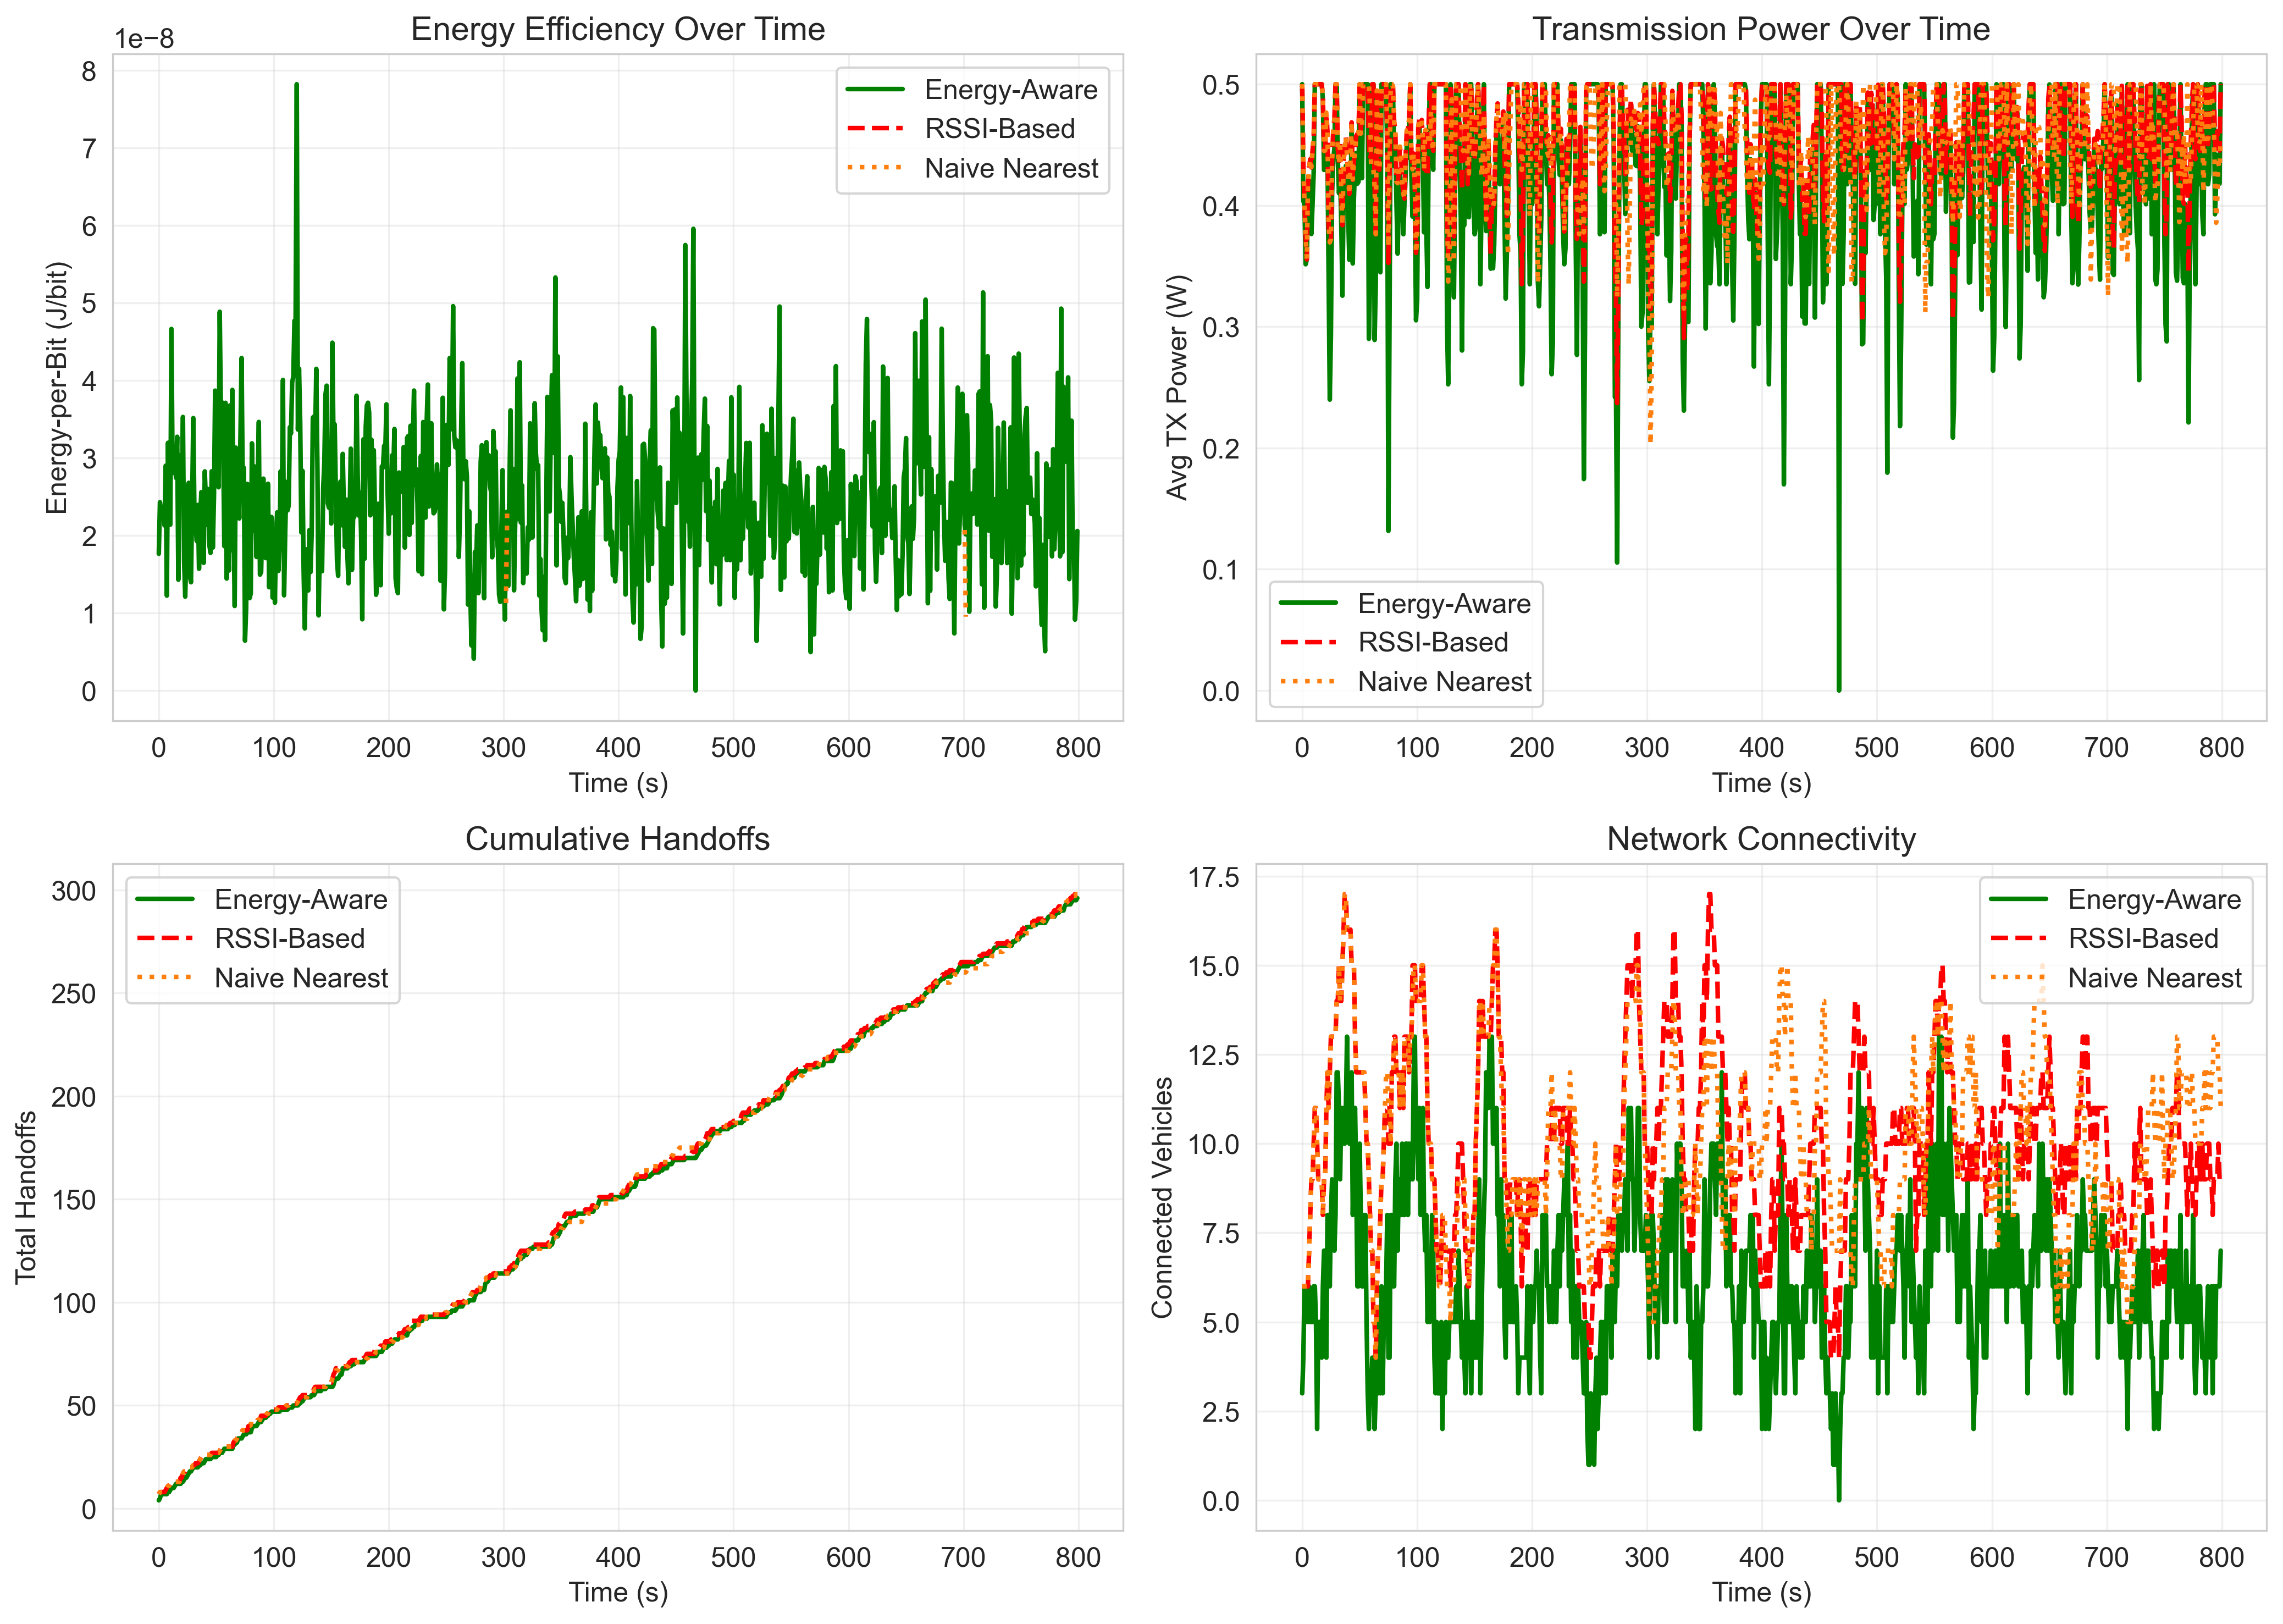
\includegraphics[width=\columnwidth]{results/energy_comparison.png}
\caption{Energy comparison dashboard across algorithms over time.}
\label{fig:energy_comparison}
\end{figure}

\begin{figure}[t]
\centering
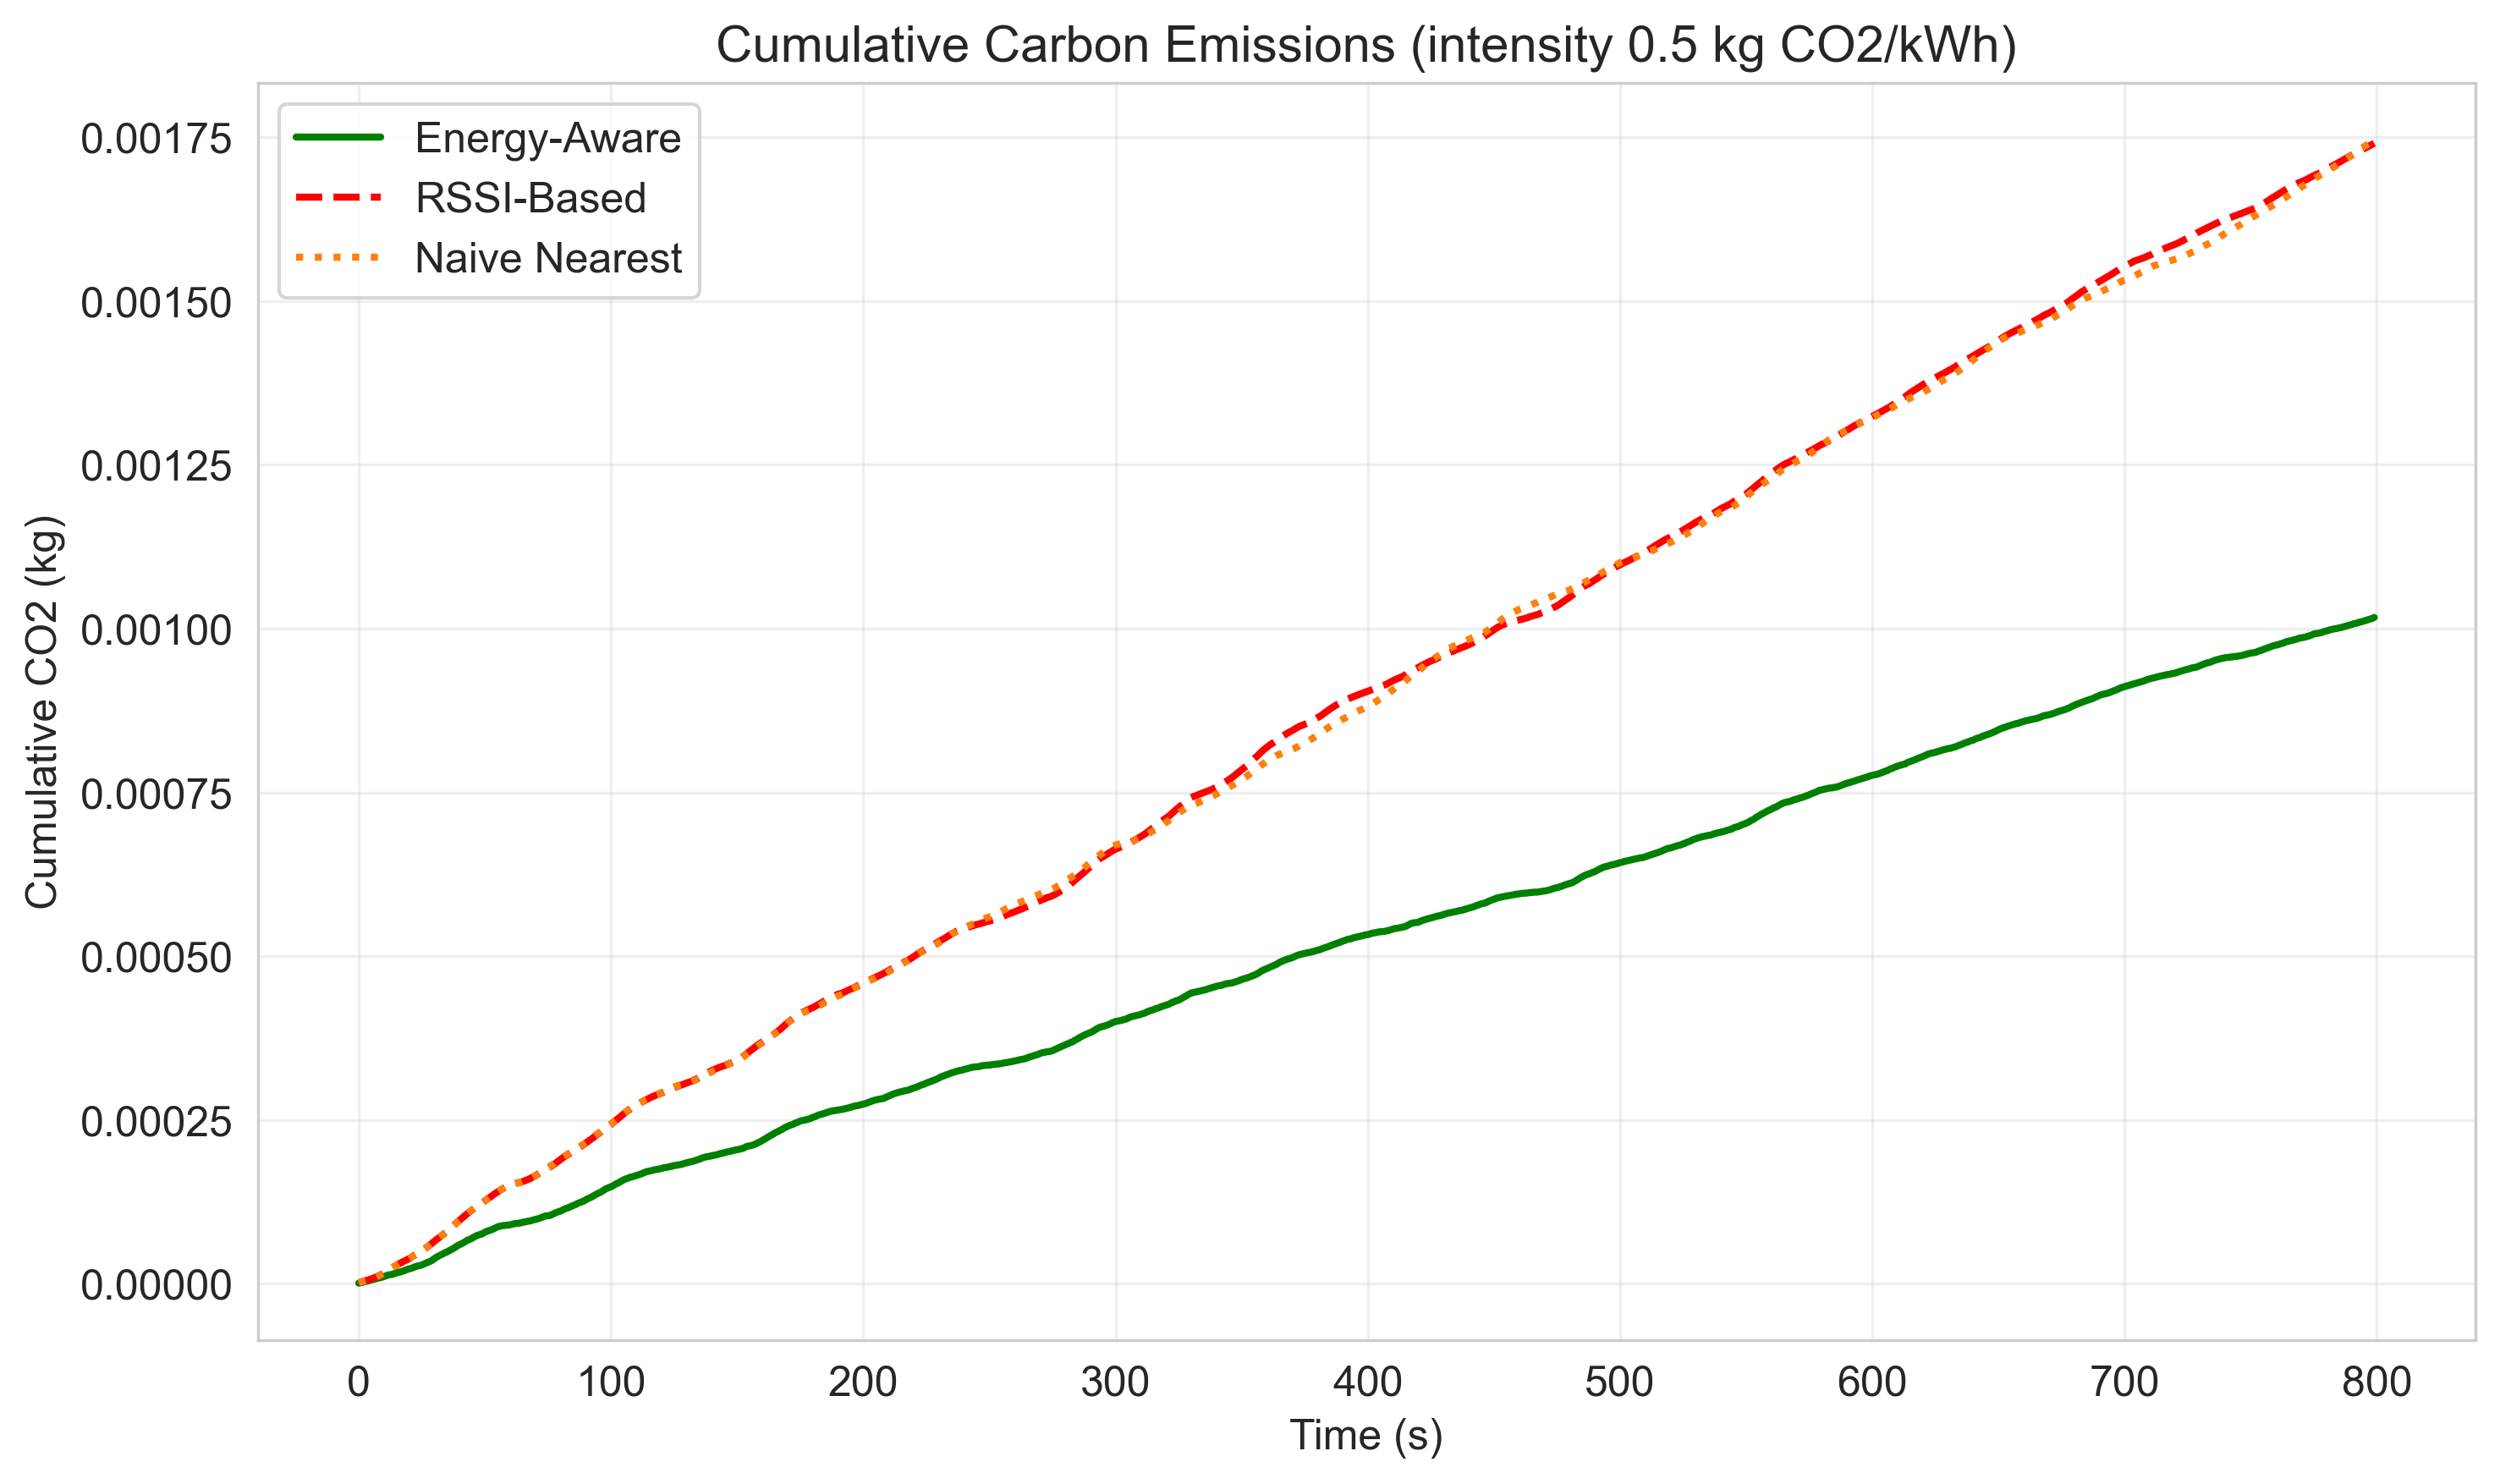
\includegraphics[width=\columnwidth]{results/cumulative_co2.png}
\caption{Cumulative CO2 emissions comparison.}
\label{fig:cumulative_co2}
\end{figure}

\begin{figure}[t]
\centering
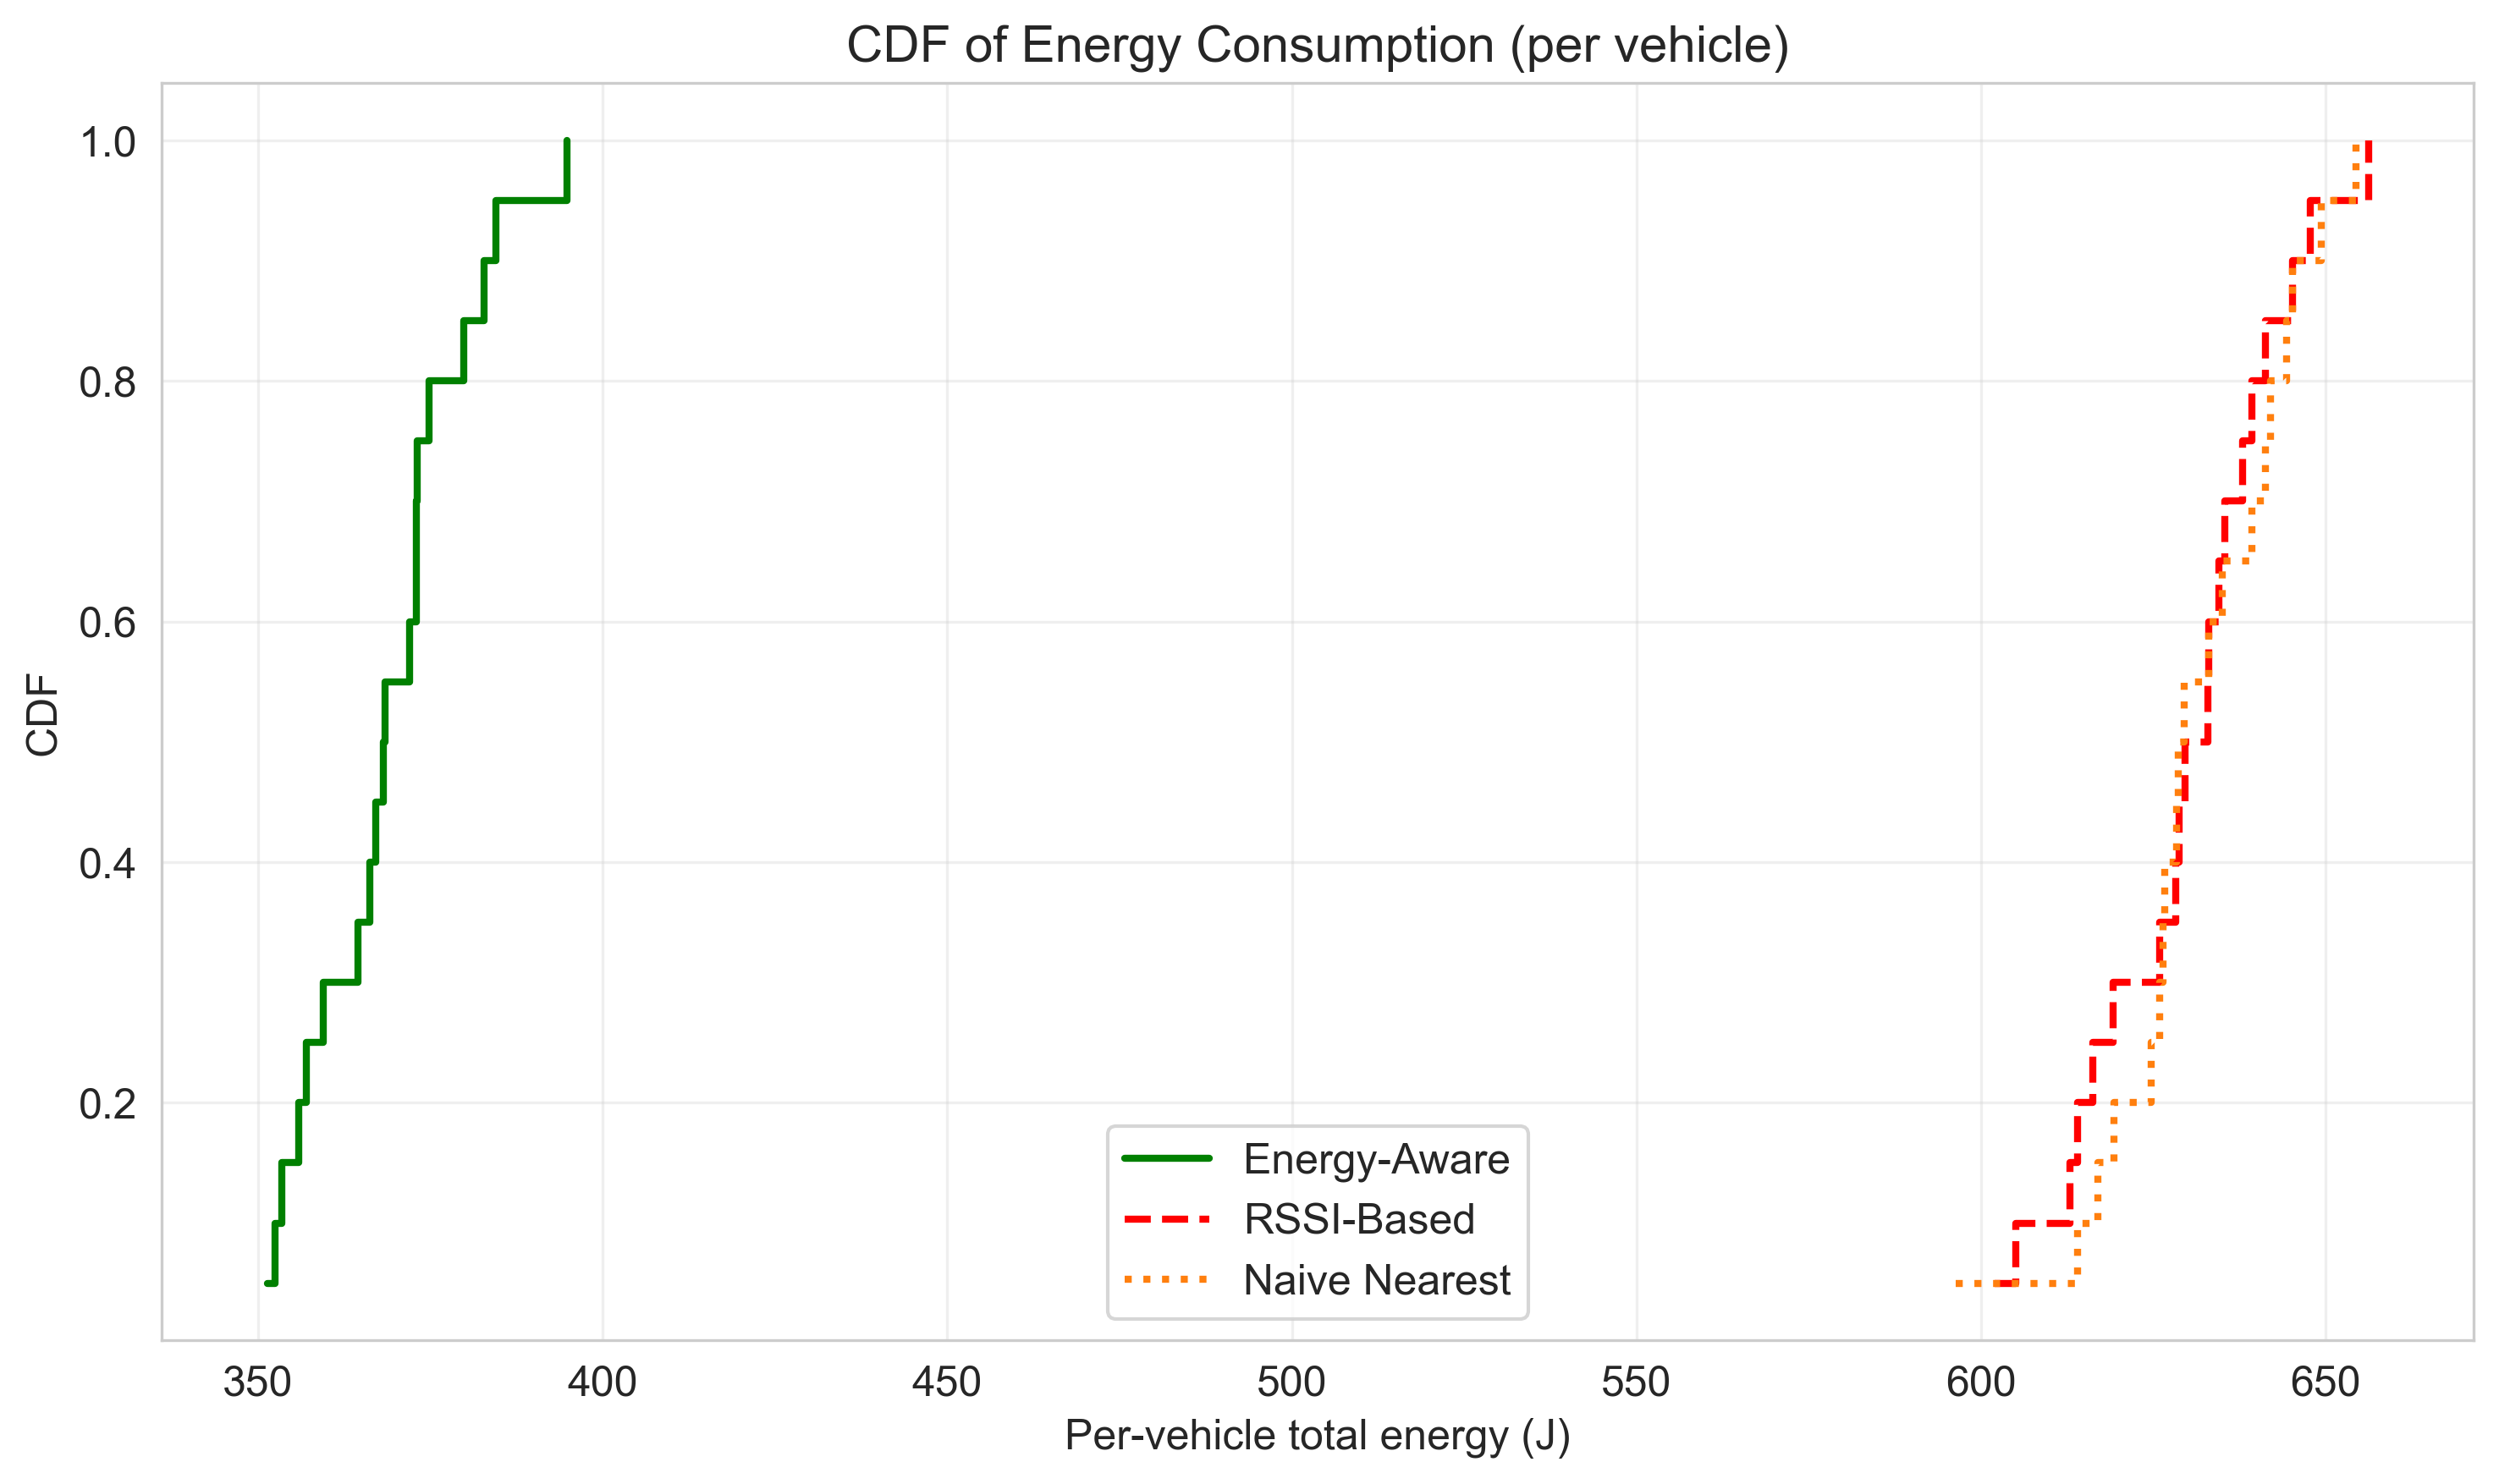
\includegraphics[width=\columnwidth]{results/energy_per_vehicle_cdf.png}
\caption{Empirical CDF of per-vehicle energy consumption.}
\label{fig:energy_per_vehicle_cdf}
\end{figure}

\begin{figure}[t]
\centering
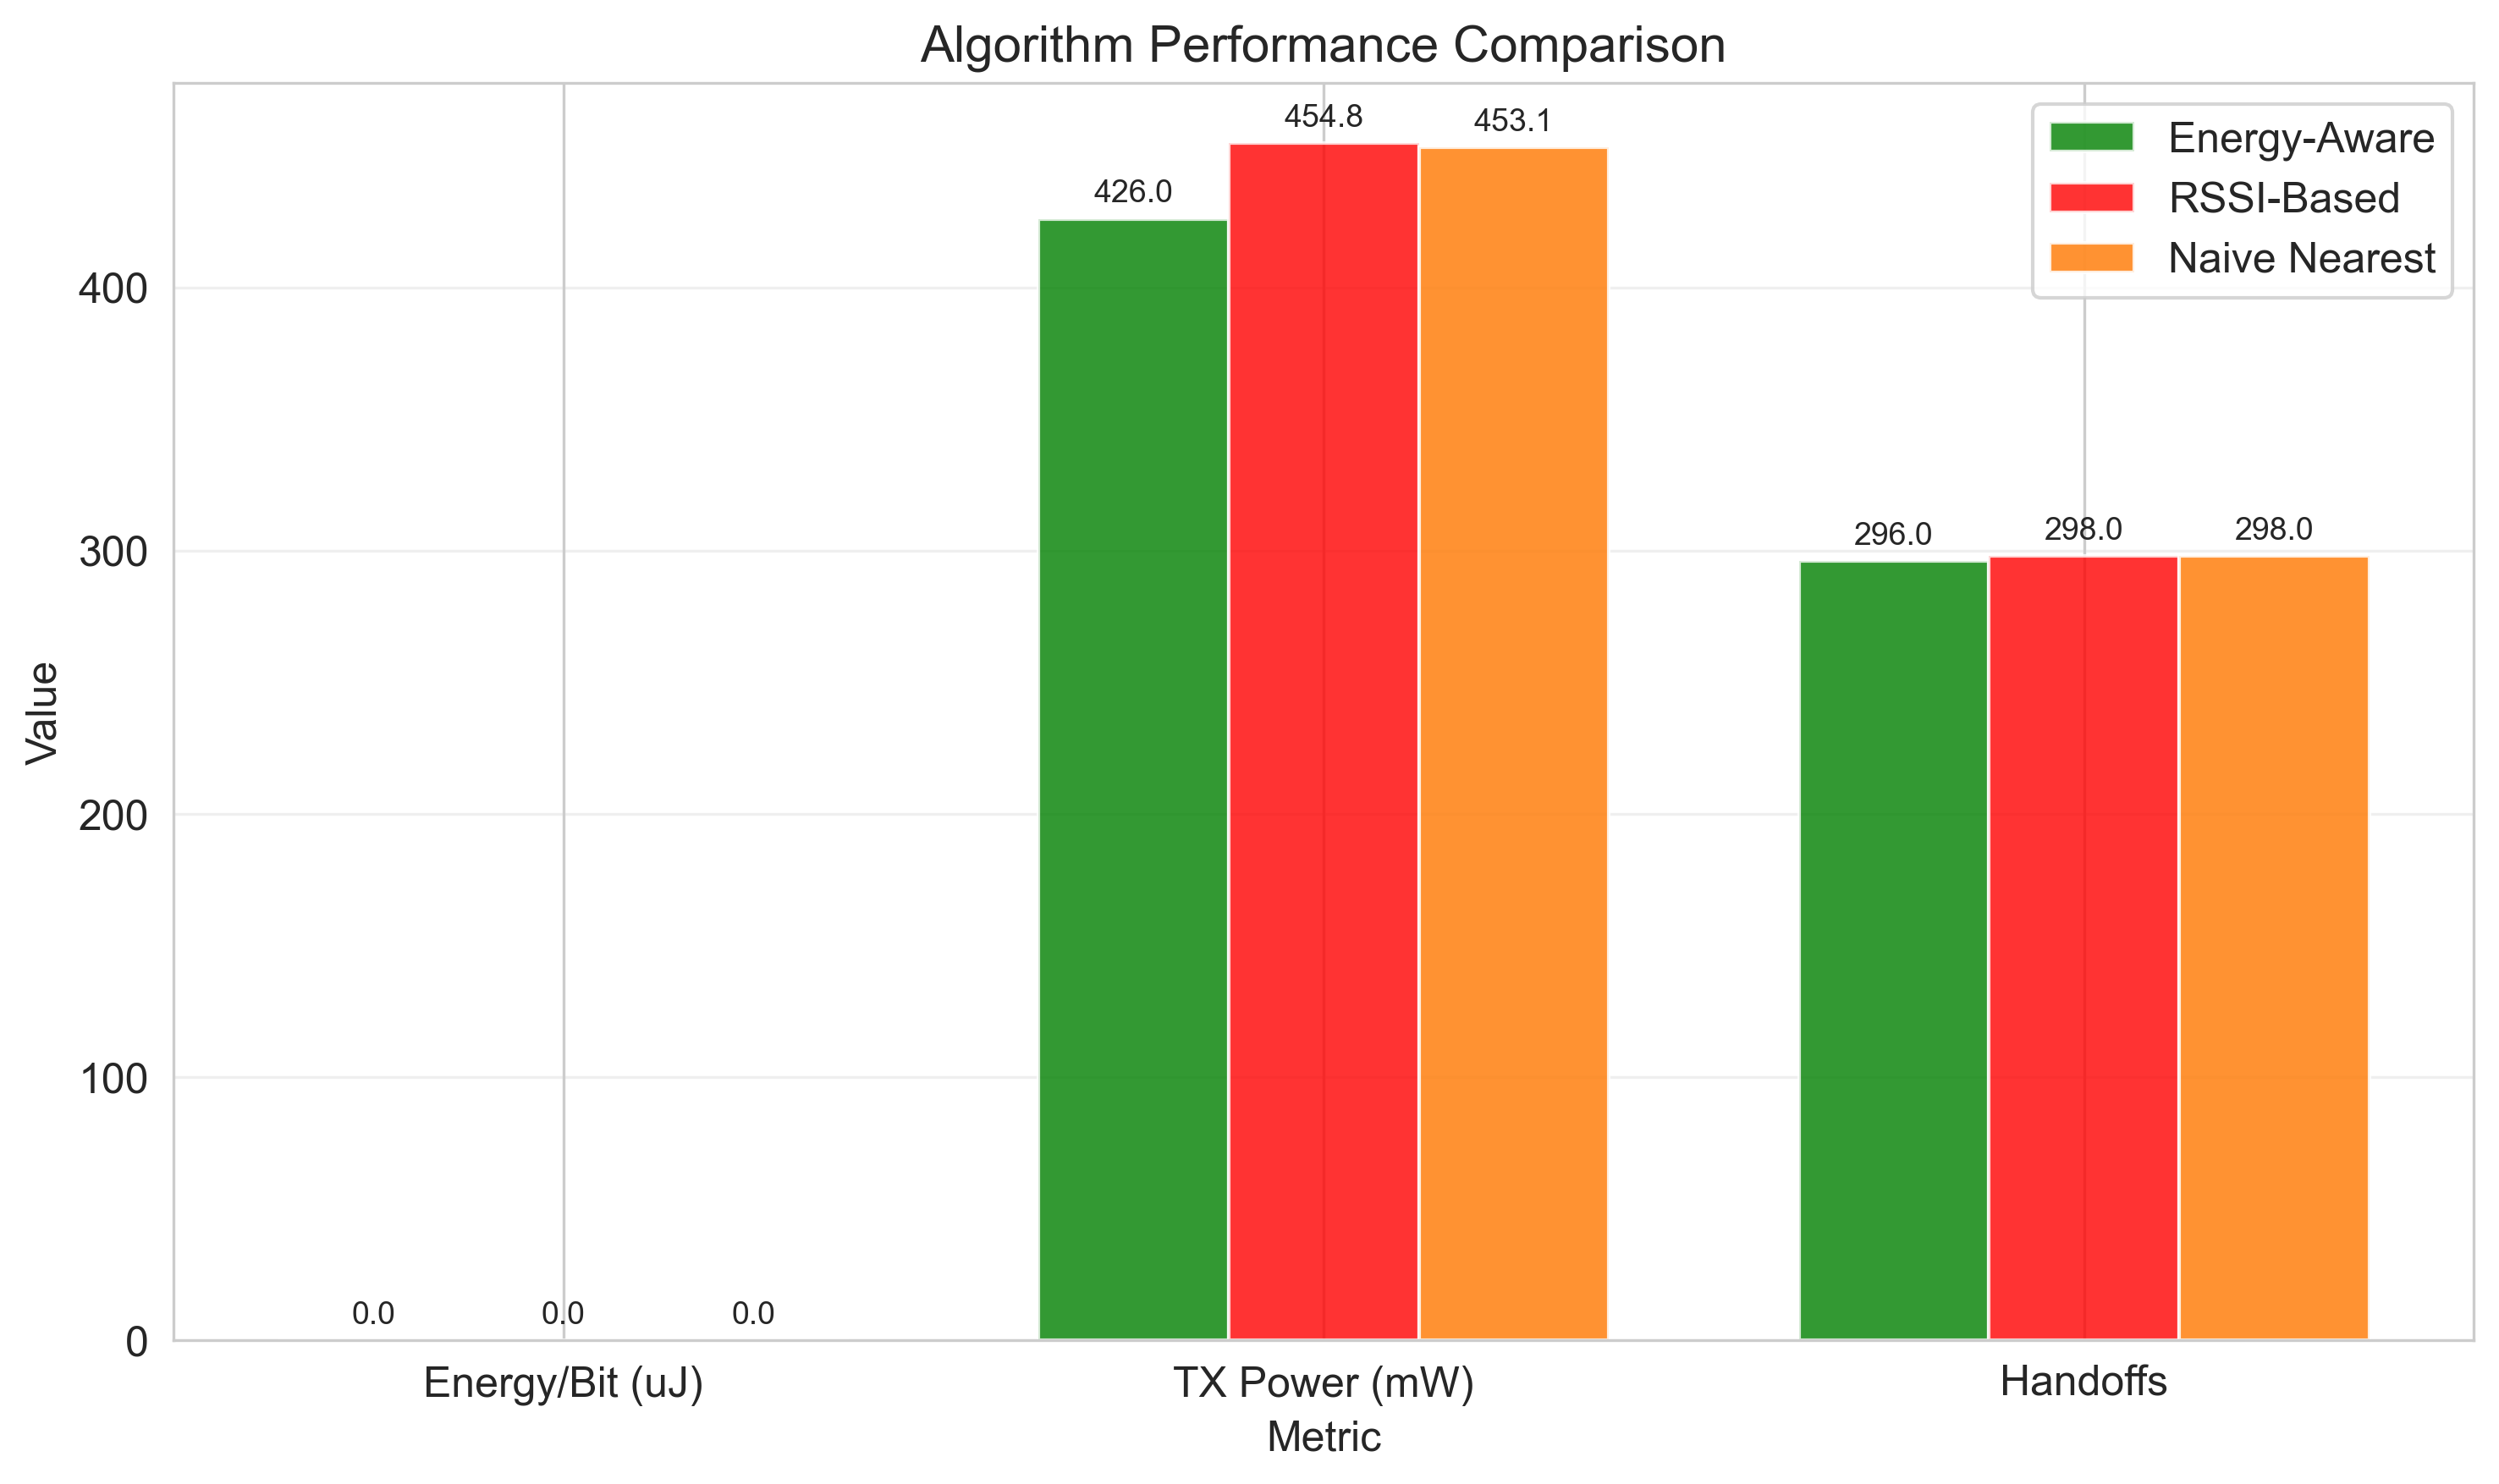
\includegraphics[width=\columnwidth]{results/bar_comparison.png}
\caption{Bar comparison of EPB, TX power, and handoffs.}
\label{fig:bar_comparison}
\end{figure}

\begin{figure}[t]
\centering
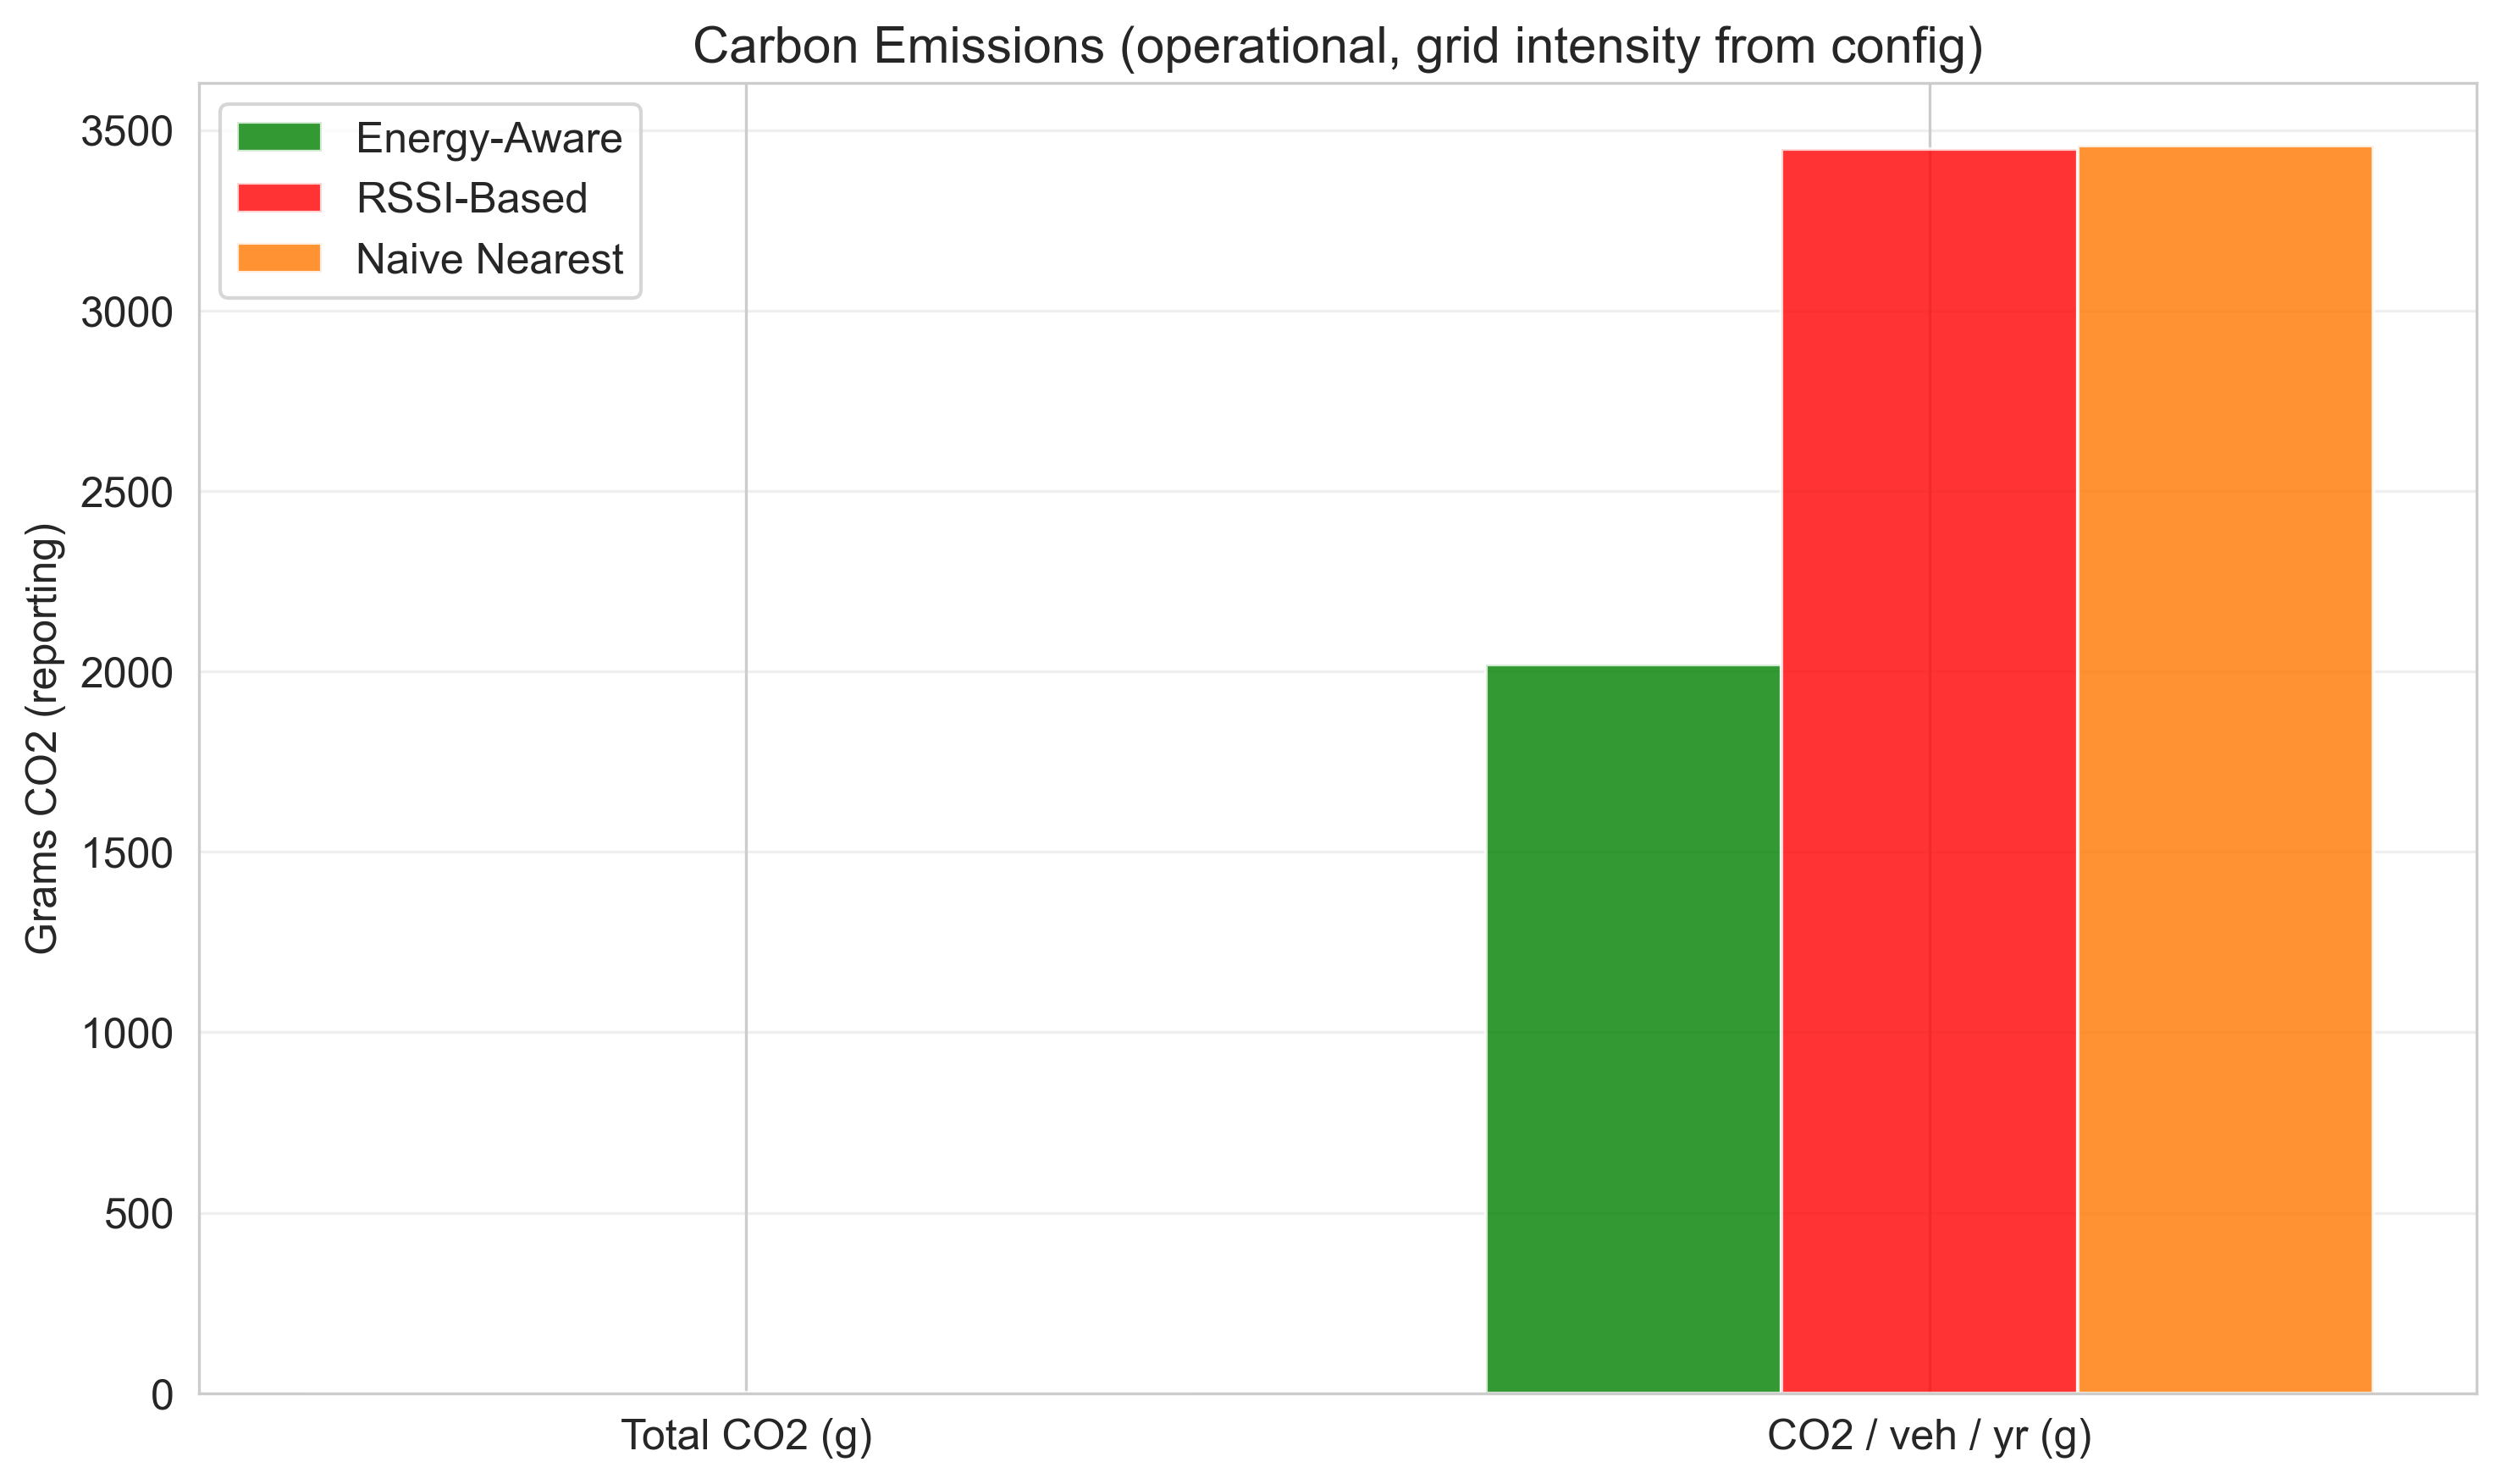
\includegraphics[width=\columnwidth]{results/bar_co2_comparison.png}
\caption{Bar comparison of total and per-vehicle CO2 emissions.}
\label{fig:bar_co2_comparison}
\end{figure}

\begin{figure}[t]
\centering
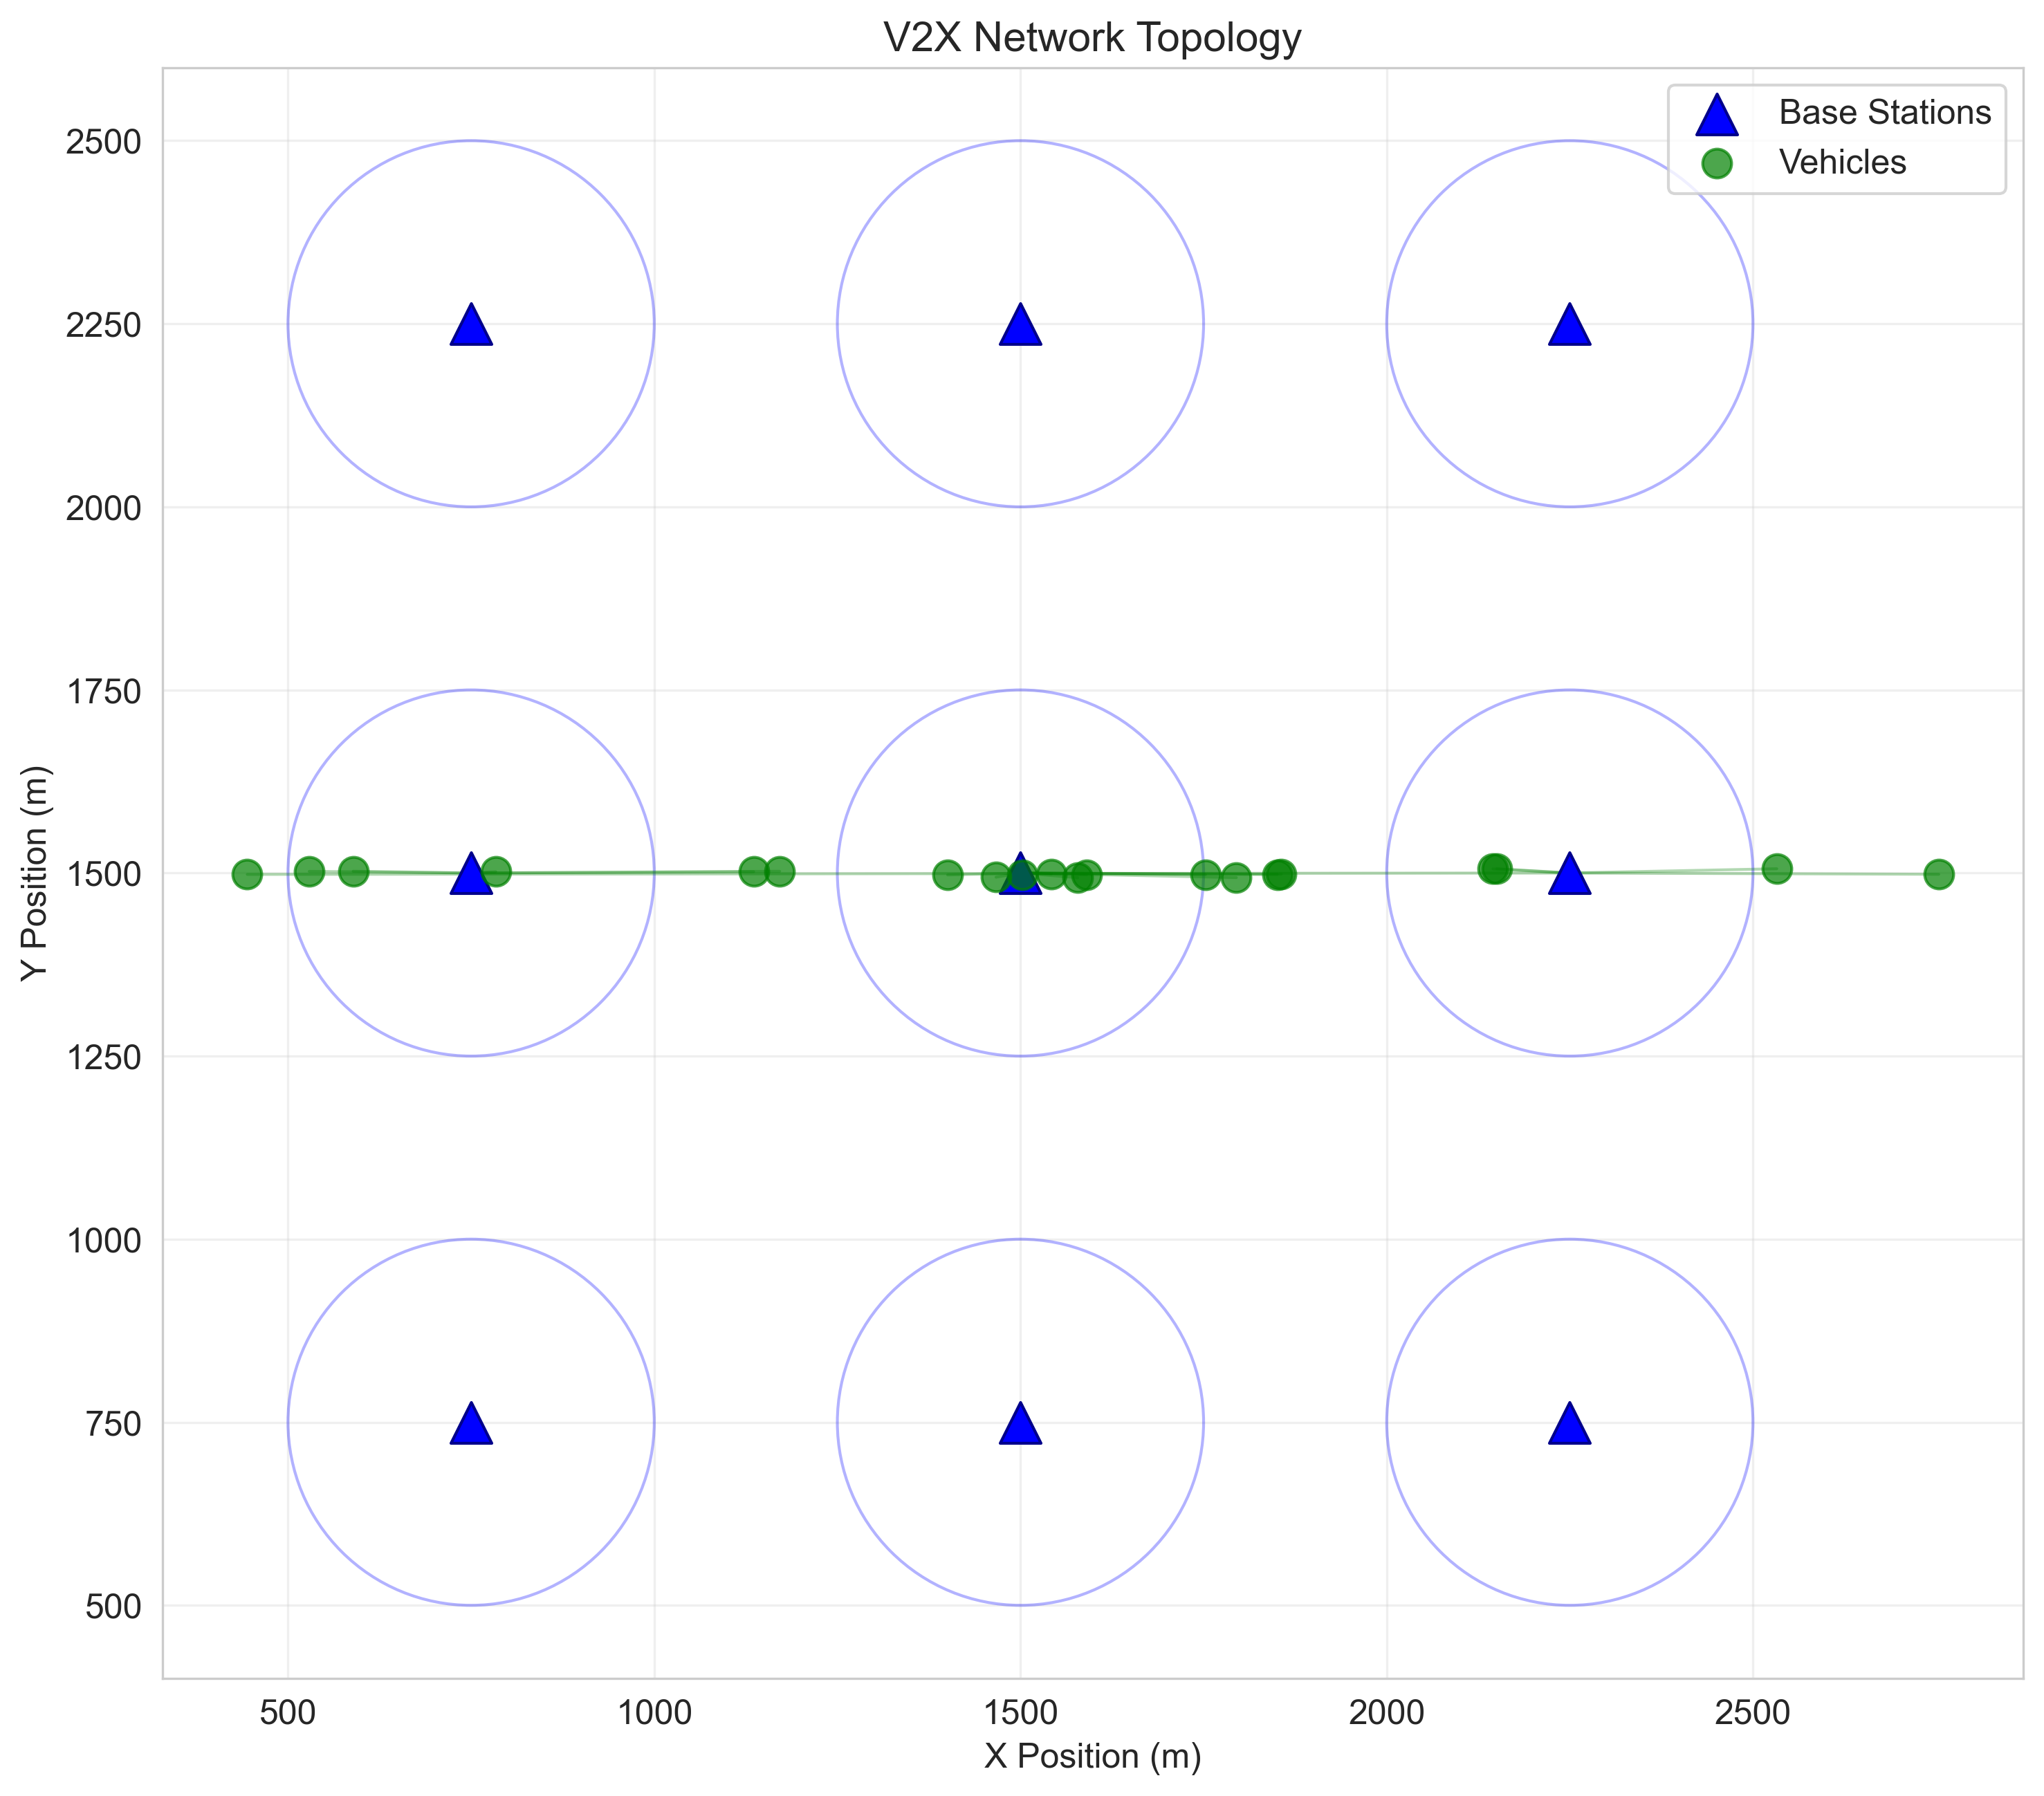
\includegraphics[width=\columnwidth]{results/network_topology.png}
\caption{Network topology and serving-BS associations snapshot.}
\label{fig:network_topology}
\end{figure}

\begin{figure}[t]
\centering
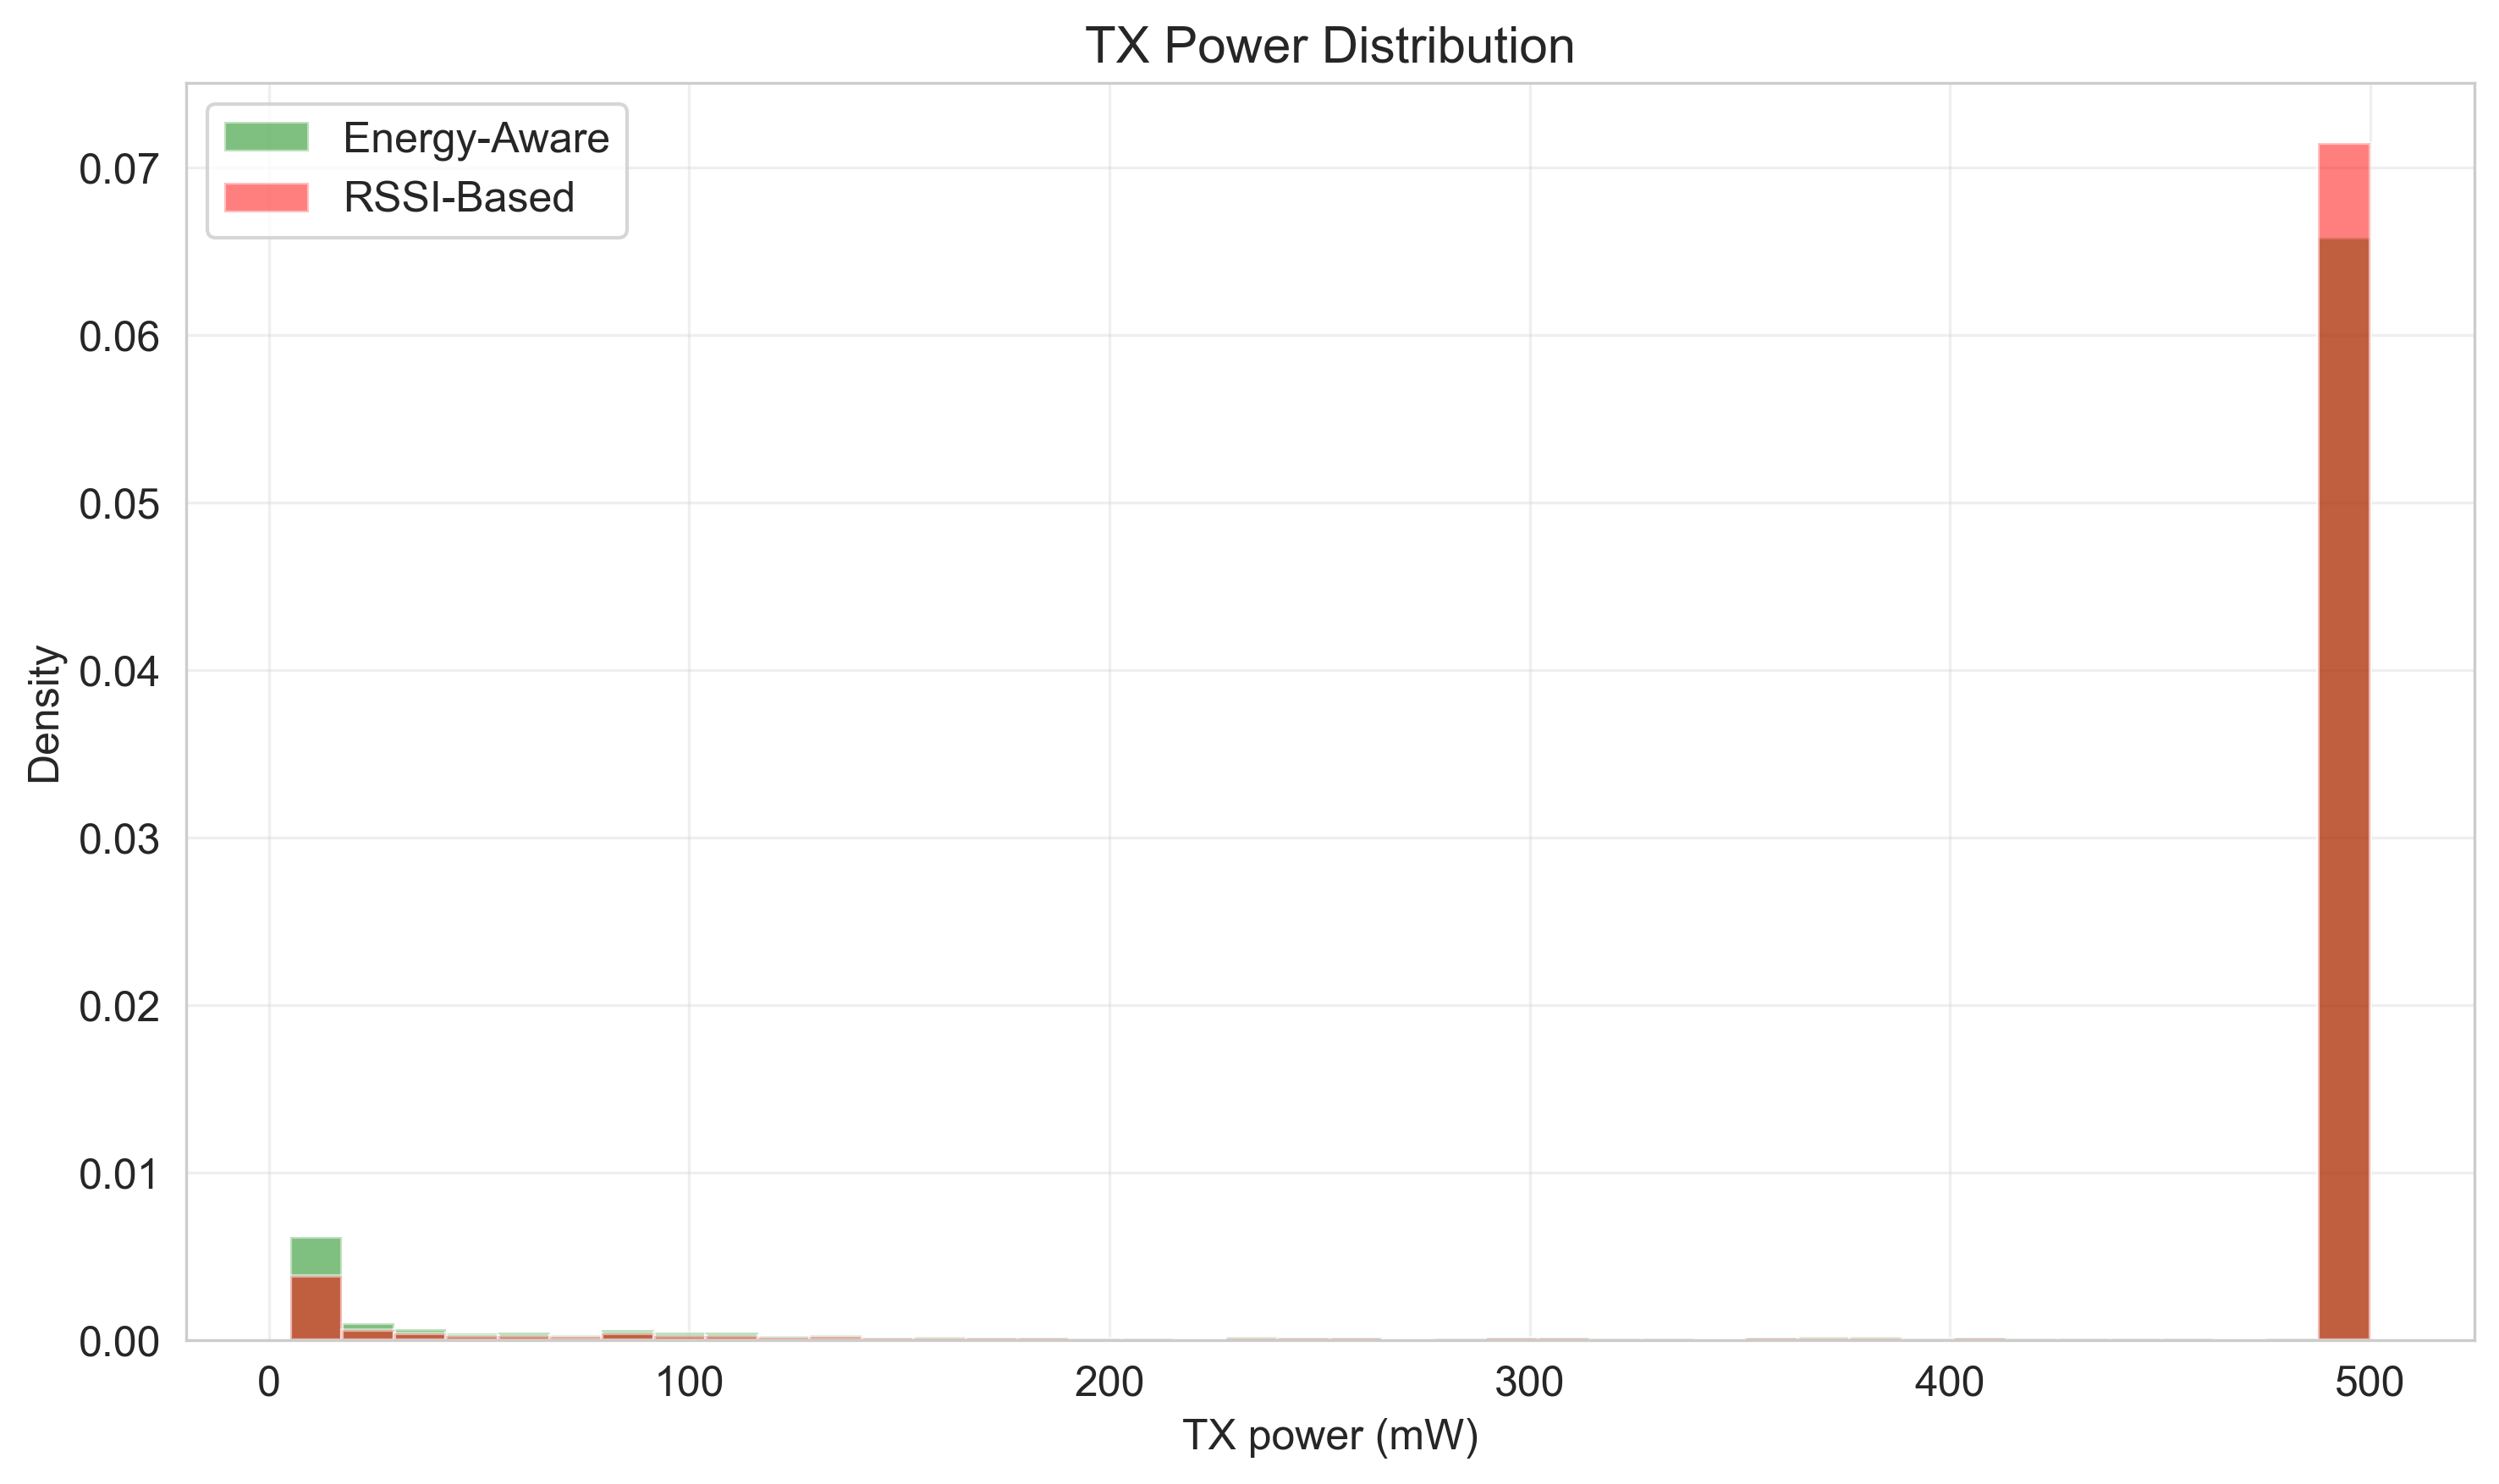
\includegraphics[width=\columnwidth]{results/tx_power_distribution.png}
\caption{Transmit power distribution for compared handoff policies.}
\label{fig:tx_power_distribution}
\end{figure}

\begin{figure}[t]
\centering
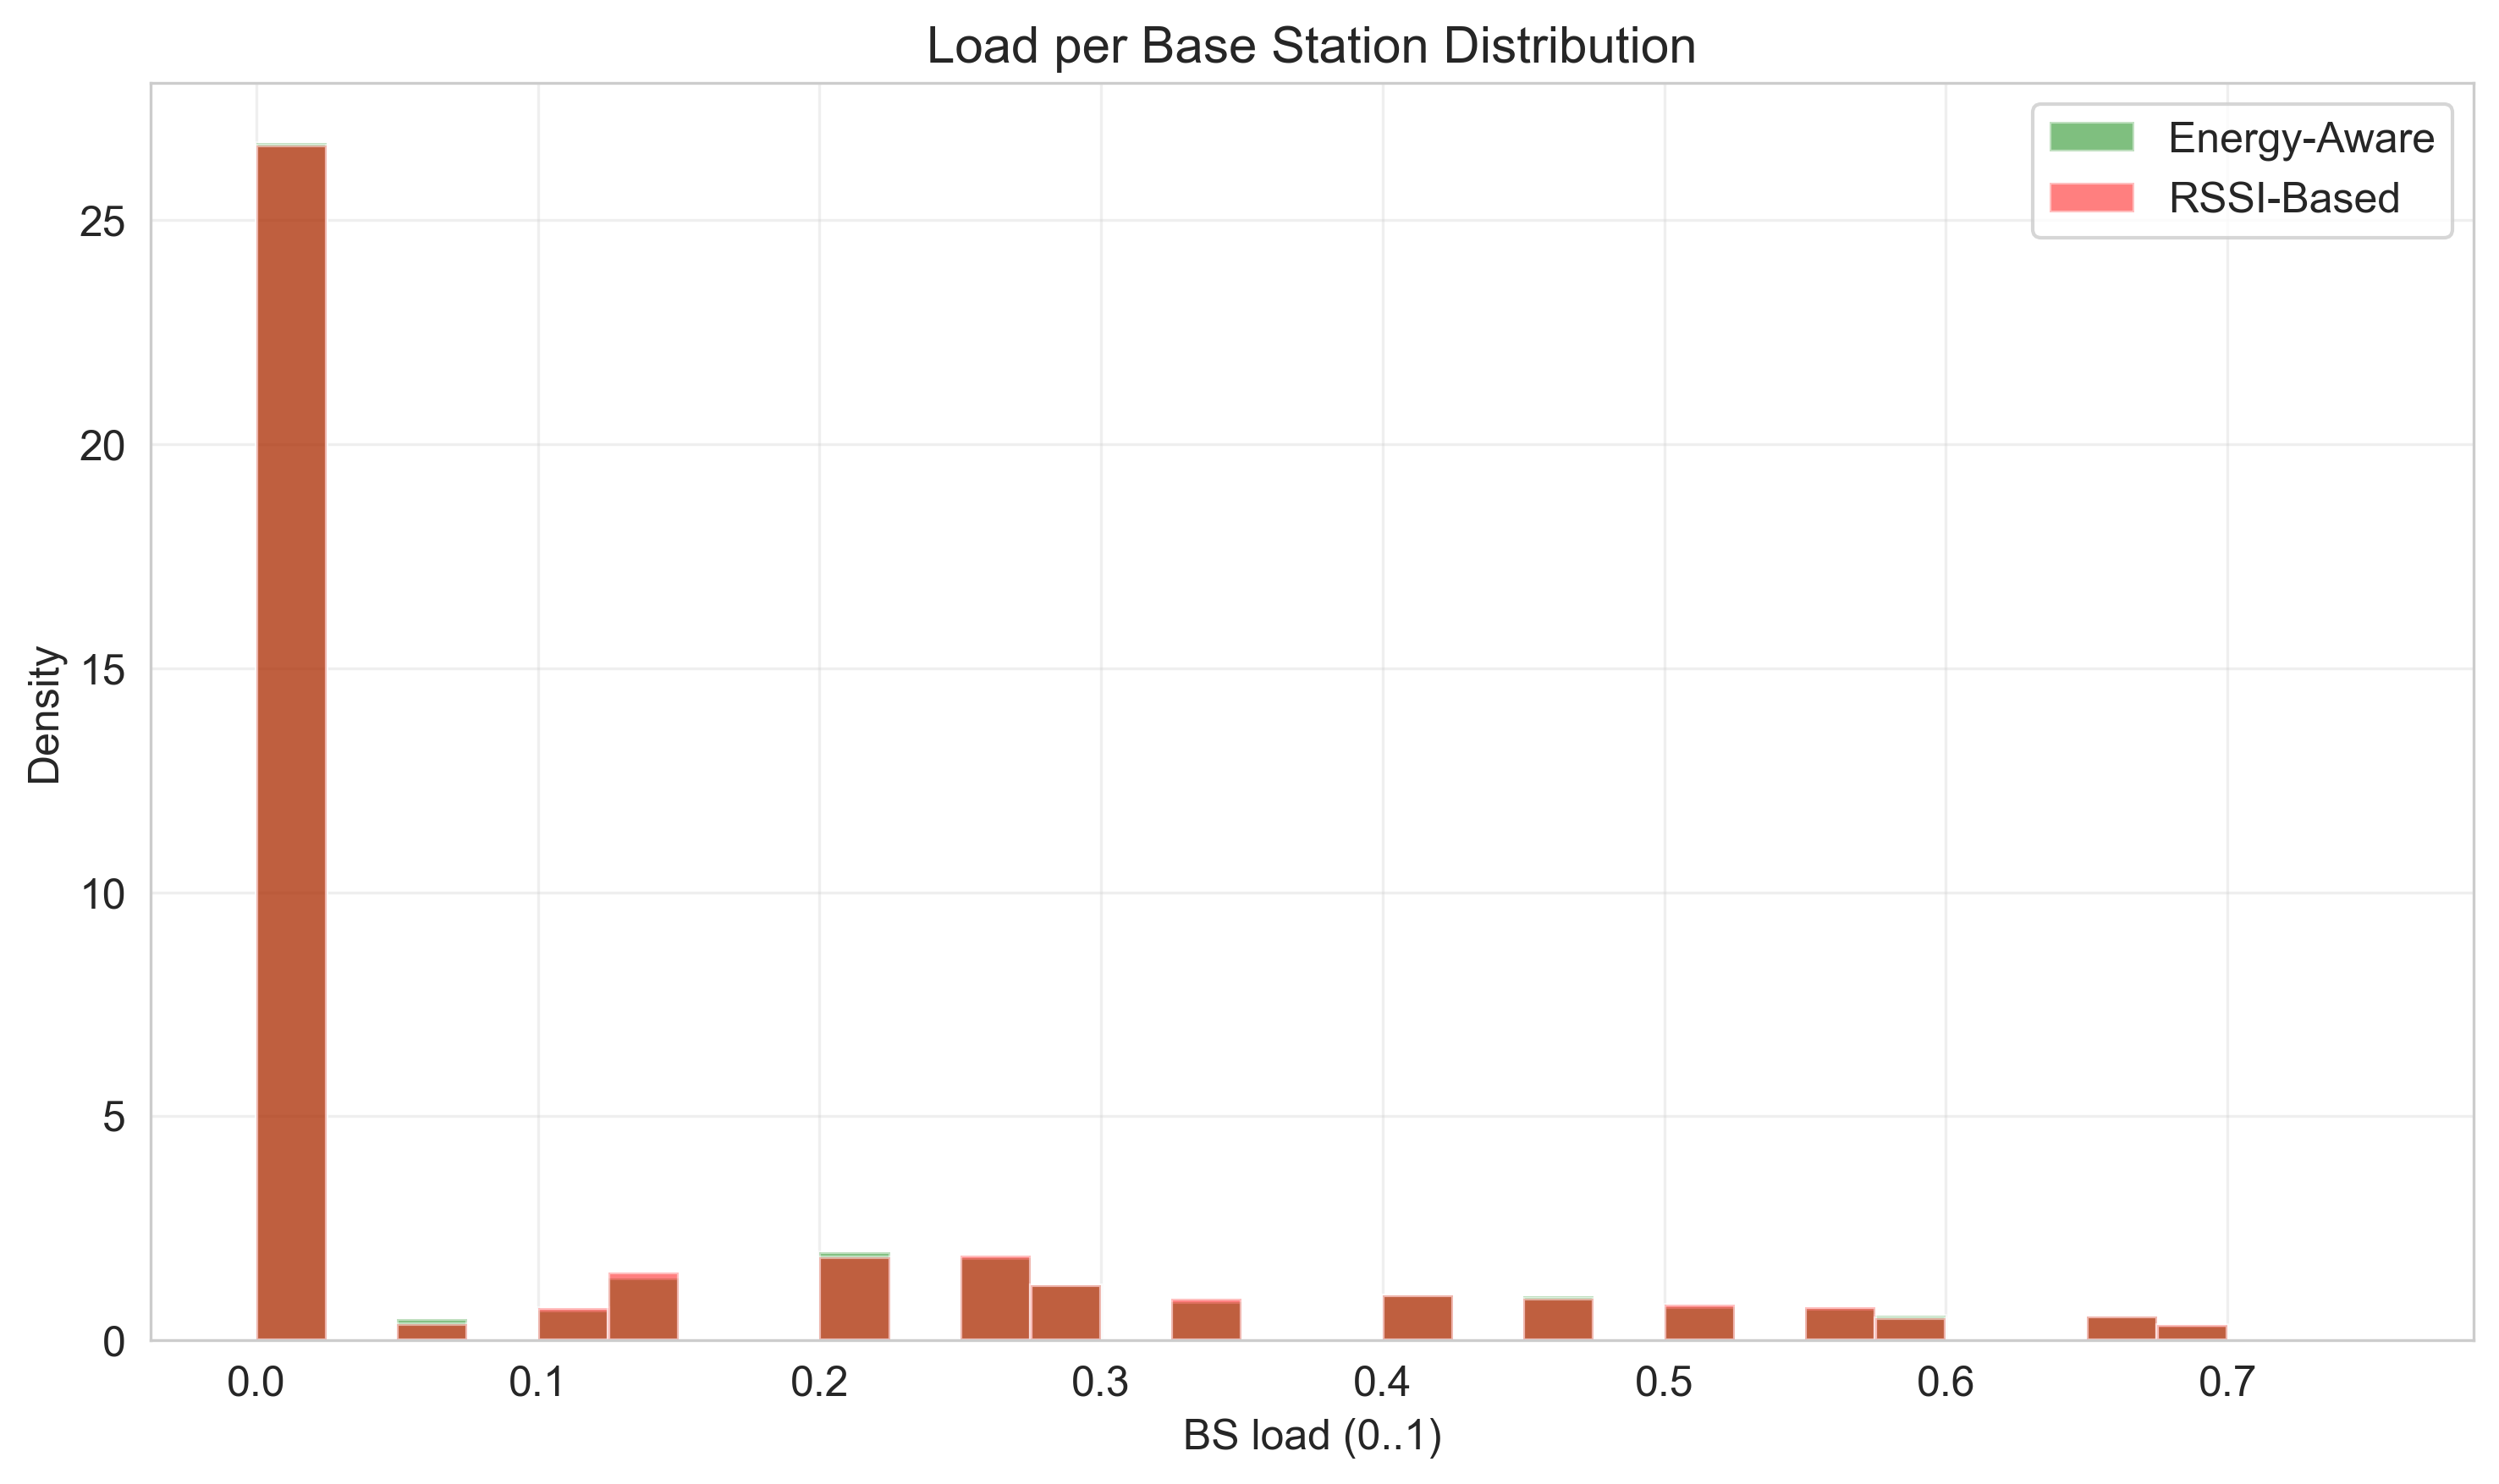
\includegraphics[width=\columnwidth]{results/bs_load_distribution.png}
\caption{Base-station load distribution under different policies.}
\label{fig:bs_load_distribution}
\end{figure}

\begin{figure}[t]
\centering
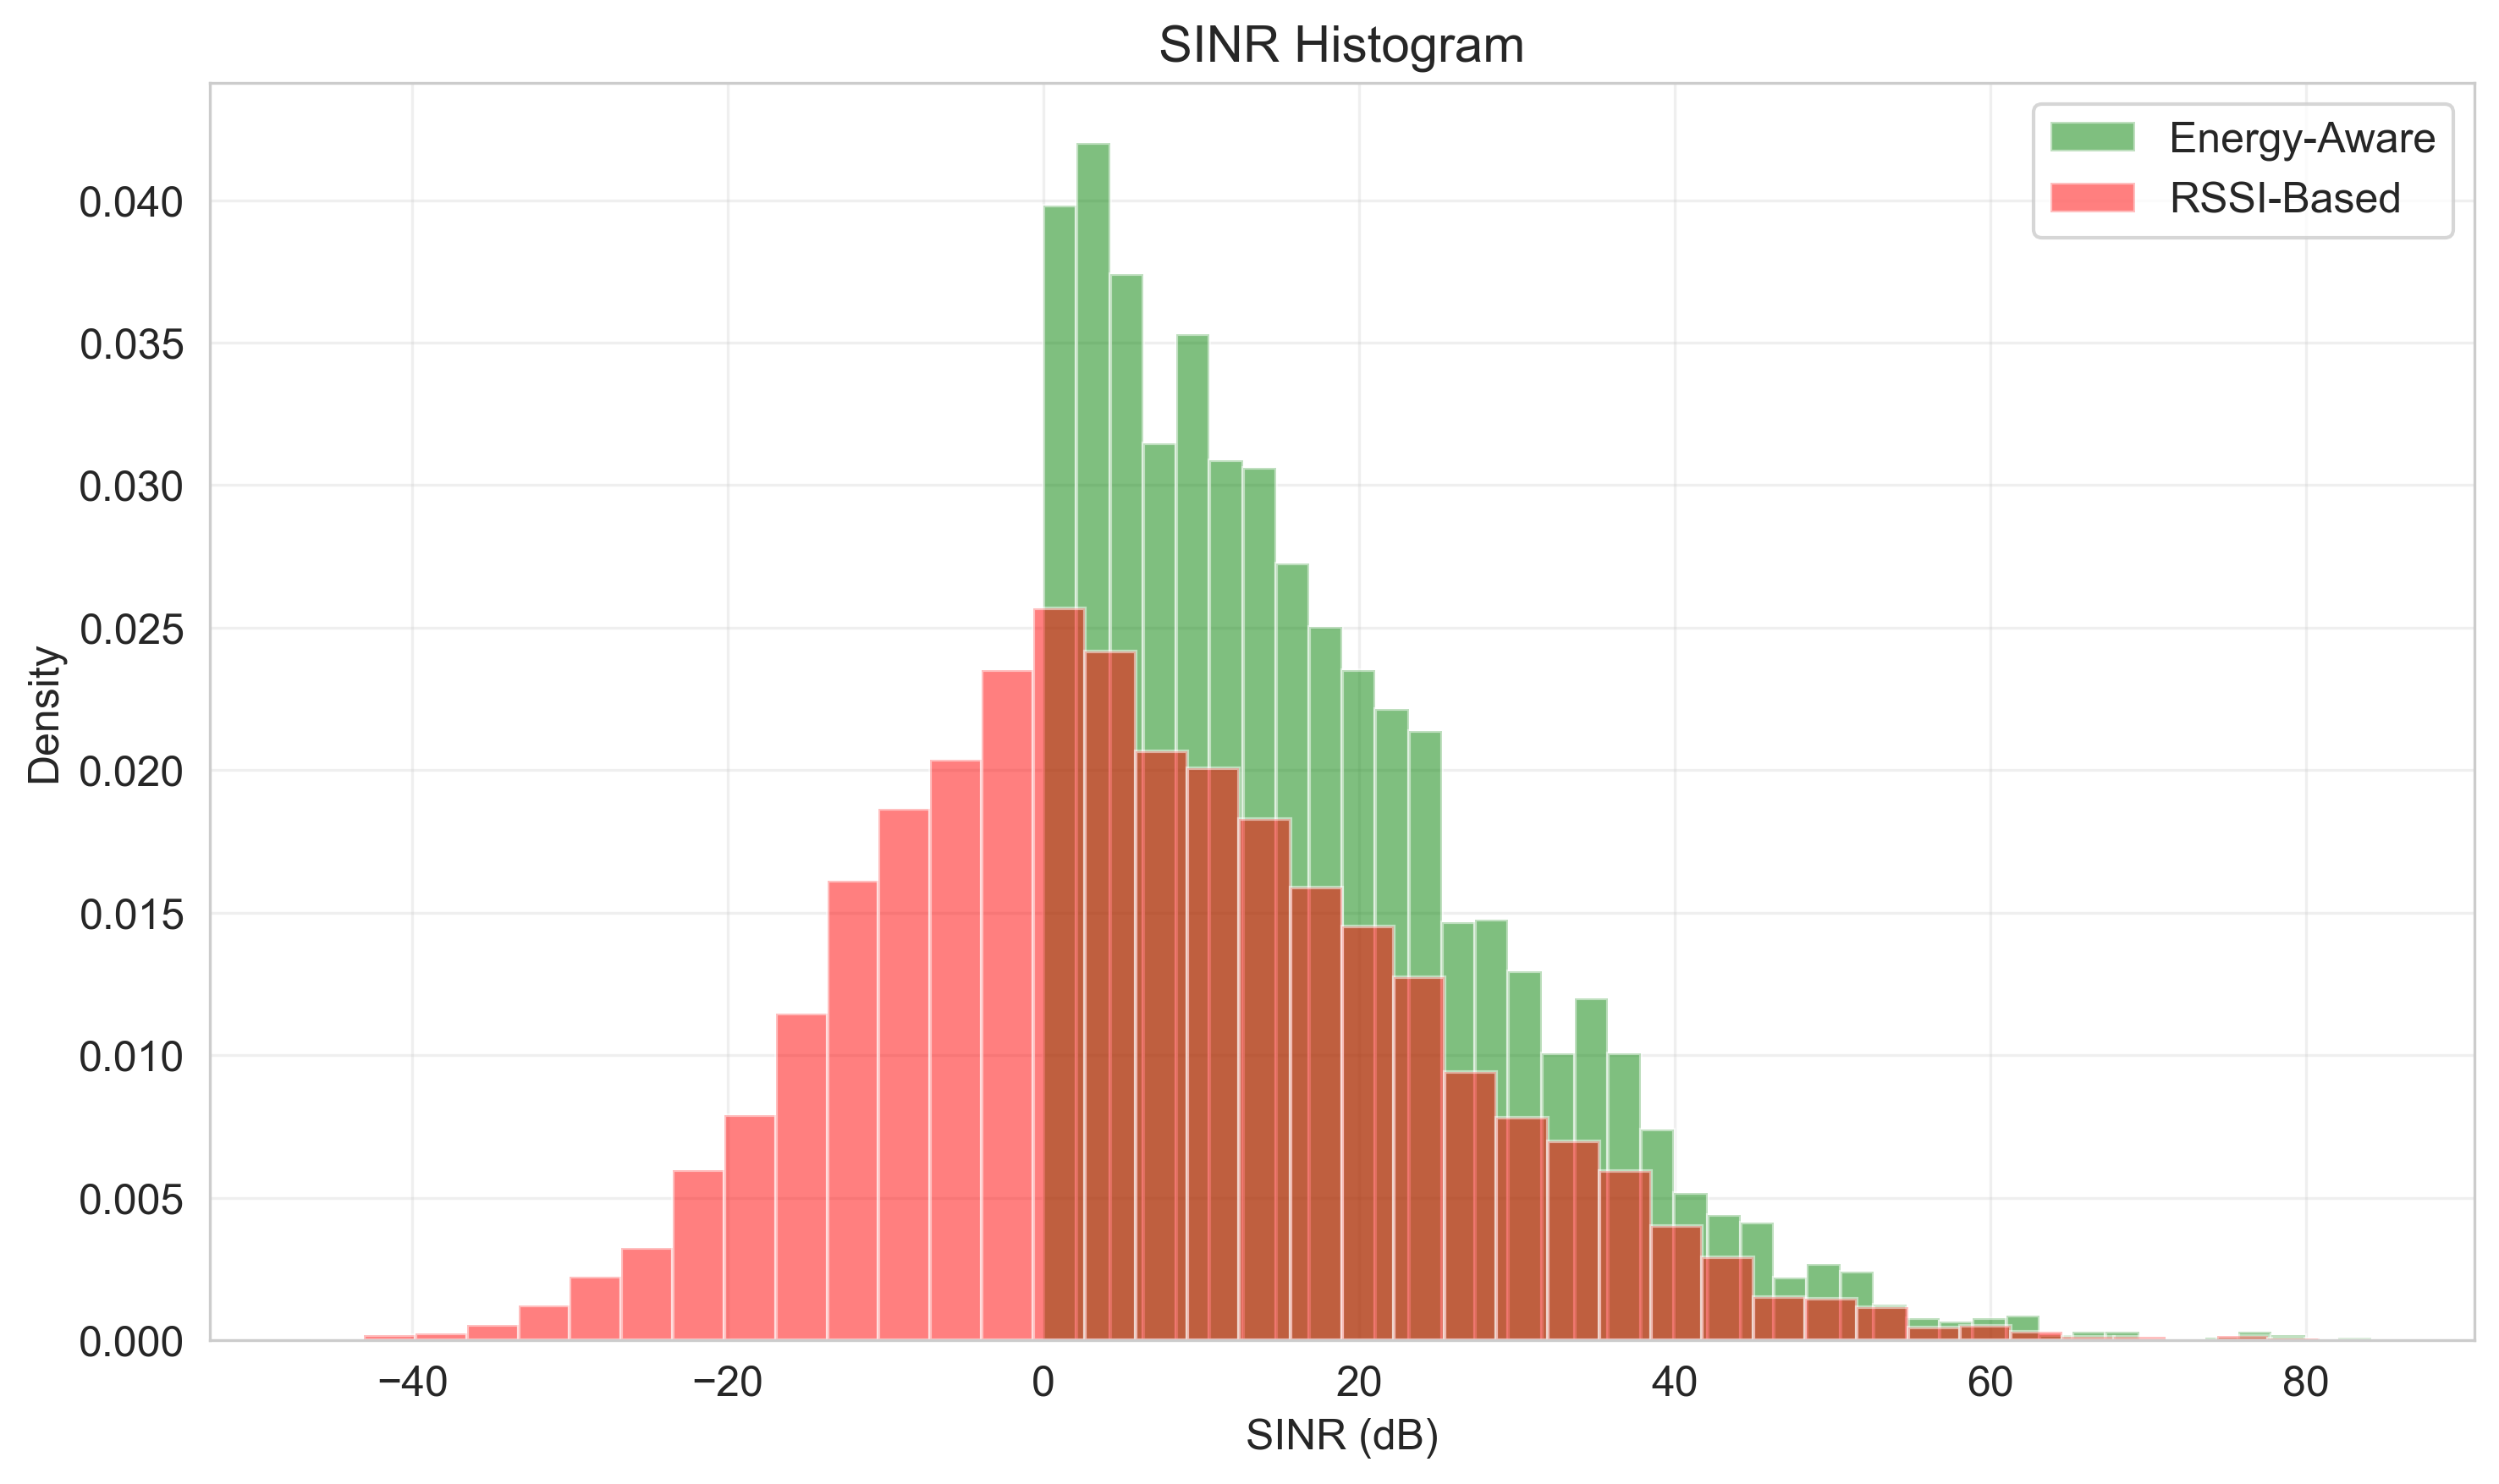
\includegraphics[width=\columnwidth]{results/sinr_histogram.png}
\caption{SINR histogram comparison across algorithms.}
\label{fig:sinr_histogram}
\end{figure}



\section{\texttt{main.py} experiment suite: what each experiment tests}

\subsection{1. Baseline multi-seed comparison}
\begin{itemize}
\item Seeds: \texttt{[42, 123, 456, 789, 1011]}.
\item For each seed:
\item Run \texttt{V2XSimulator.run\_comparison()}.
\item Store \texttt{results\_list} with per-seed comparison.
\end{itemize}

\paragraph*{Metrics computed across seeds}
\begin{itemize}
\item Energy saving vs RSSI/SINR/load-aware RSSI in EPB.
\item Energy saving vs RSSI in total J.
\item Handoff reduction vs RSSI.
\item Energy saving vs naive.
\item RSSI vs naive energy improvement.
\item Multi-seed averages of total energy for each algorithm.
\item Multi-seed averages for:
\item Throughput (avg, p5),
\item Outage probability,
\item Ping-pong rate,
\item Handoff delay per vehicle,
\item Service availability (avg, p5).
\end{itemize}

\paragraph*{Paired t-tests}
\begin{itemize}
\item Since same seeds:
\item \texttt{stats.ttest\_rel(rssi\_e, ea\_e, alternative="greater")}:
\item Tests if RSSI consumes \textbf{more} energy than EA.
\item \texttt{stats.ttest\_rel(rssi\_epb, ea\_epb, alternative="greater")}:
\item Same for average EPB.
\item The p-values indicate significance of EA’s improvement.
\end{itemize}

\paragraph*{CO2 stats}
\begin{itemize}
\item Per-seed EA, RSSI, naive CO2 (kg).
\item Per-seed CO2 per vehicle per year.
\item Average + std across seeds.
\end{itemize}

\paragraph*{Constraint check}
\begin{itemize}
\item Ensure at least one seed has \textbf{>15\% EPB saving vs RSSI} in the sparse scenario (as a “target” scenario).
\item Check \texttt{energy\_aware\_handoffs\_leq\_rssi} across seeds.
\end{itemize}


\subsection{2. Scalability vs number of vehicles: \texttt{run_scaling_experiment}}
\begin{itemize}
\item Vehicle counts: \texttt{[20, 50, 100, 200]}.
\item For each count:
\item Create a config copying all parameters except \texttt{num\_vehicles}.
\item Run \texttt{V2XSimulator.run\_comparison()} over \texttt{SCALING\_SEEDS = [42, 123, 456]}.
\item Compute:
\item Mean / std of \texttt{energy\_saving\_percent} (EPB vs RSSI).
\item Plot:
\item \texttt{scaling\_energy\_saving\_vs\_vehicles.png}:
\item Error-bar plot: x = number of vehicles, y = energy saving vs RSSI (\%).
\item Save \texttt{scaling\_results.json} with numeric data.
\end{itemize}

\paragraph*{Goal}
\begin{itemize}
\item Show \textbf{energy-aware advantage scales} with more vehicles and isn’t just a small-load artifact.
\end{itemize}

\begin{figure}[t]
\centering
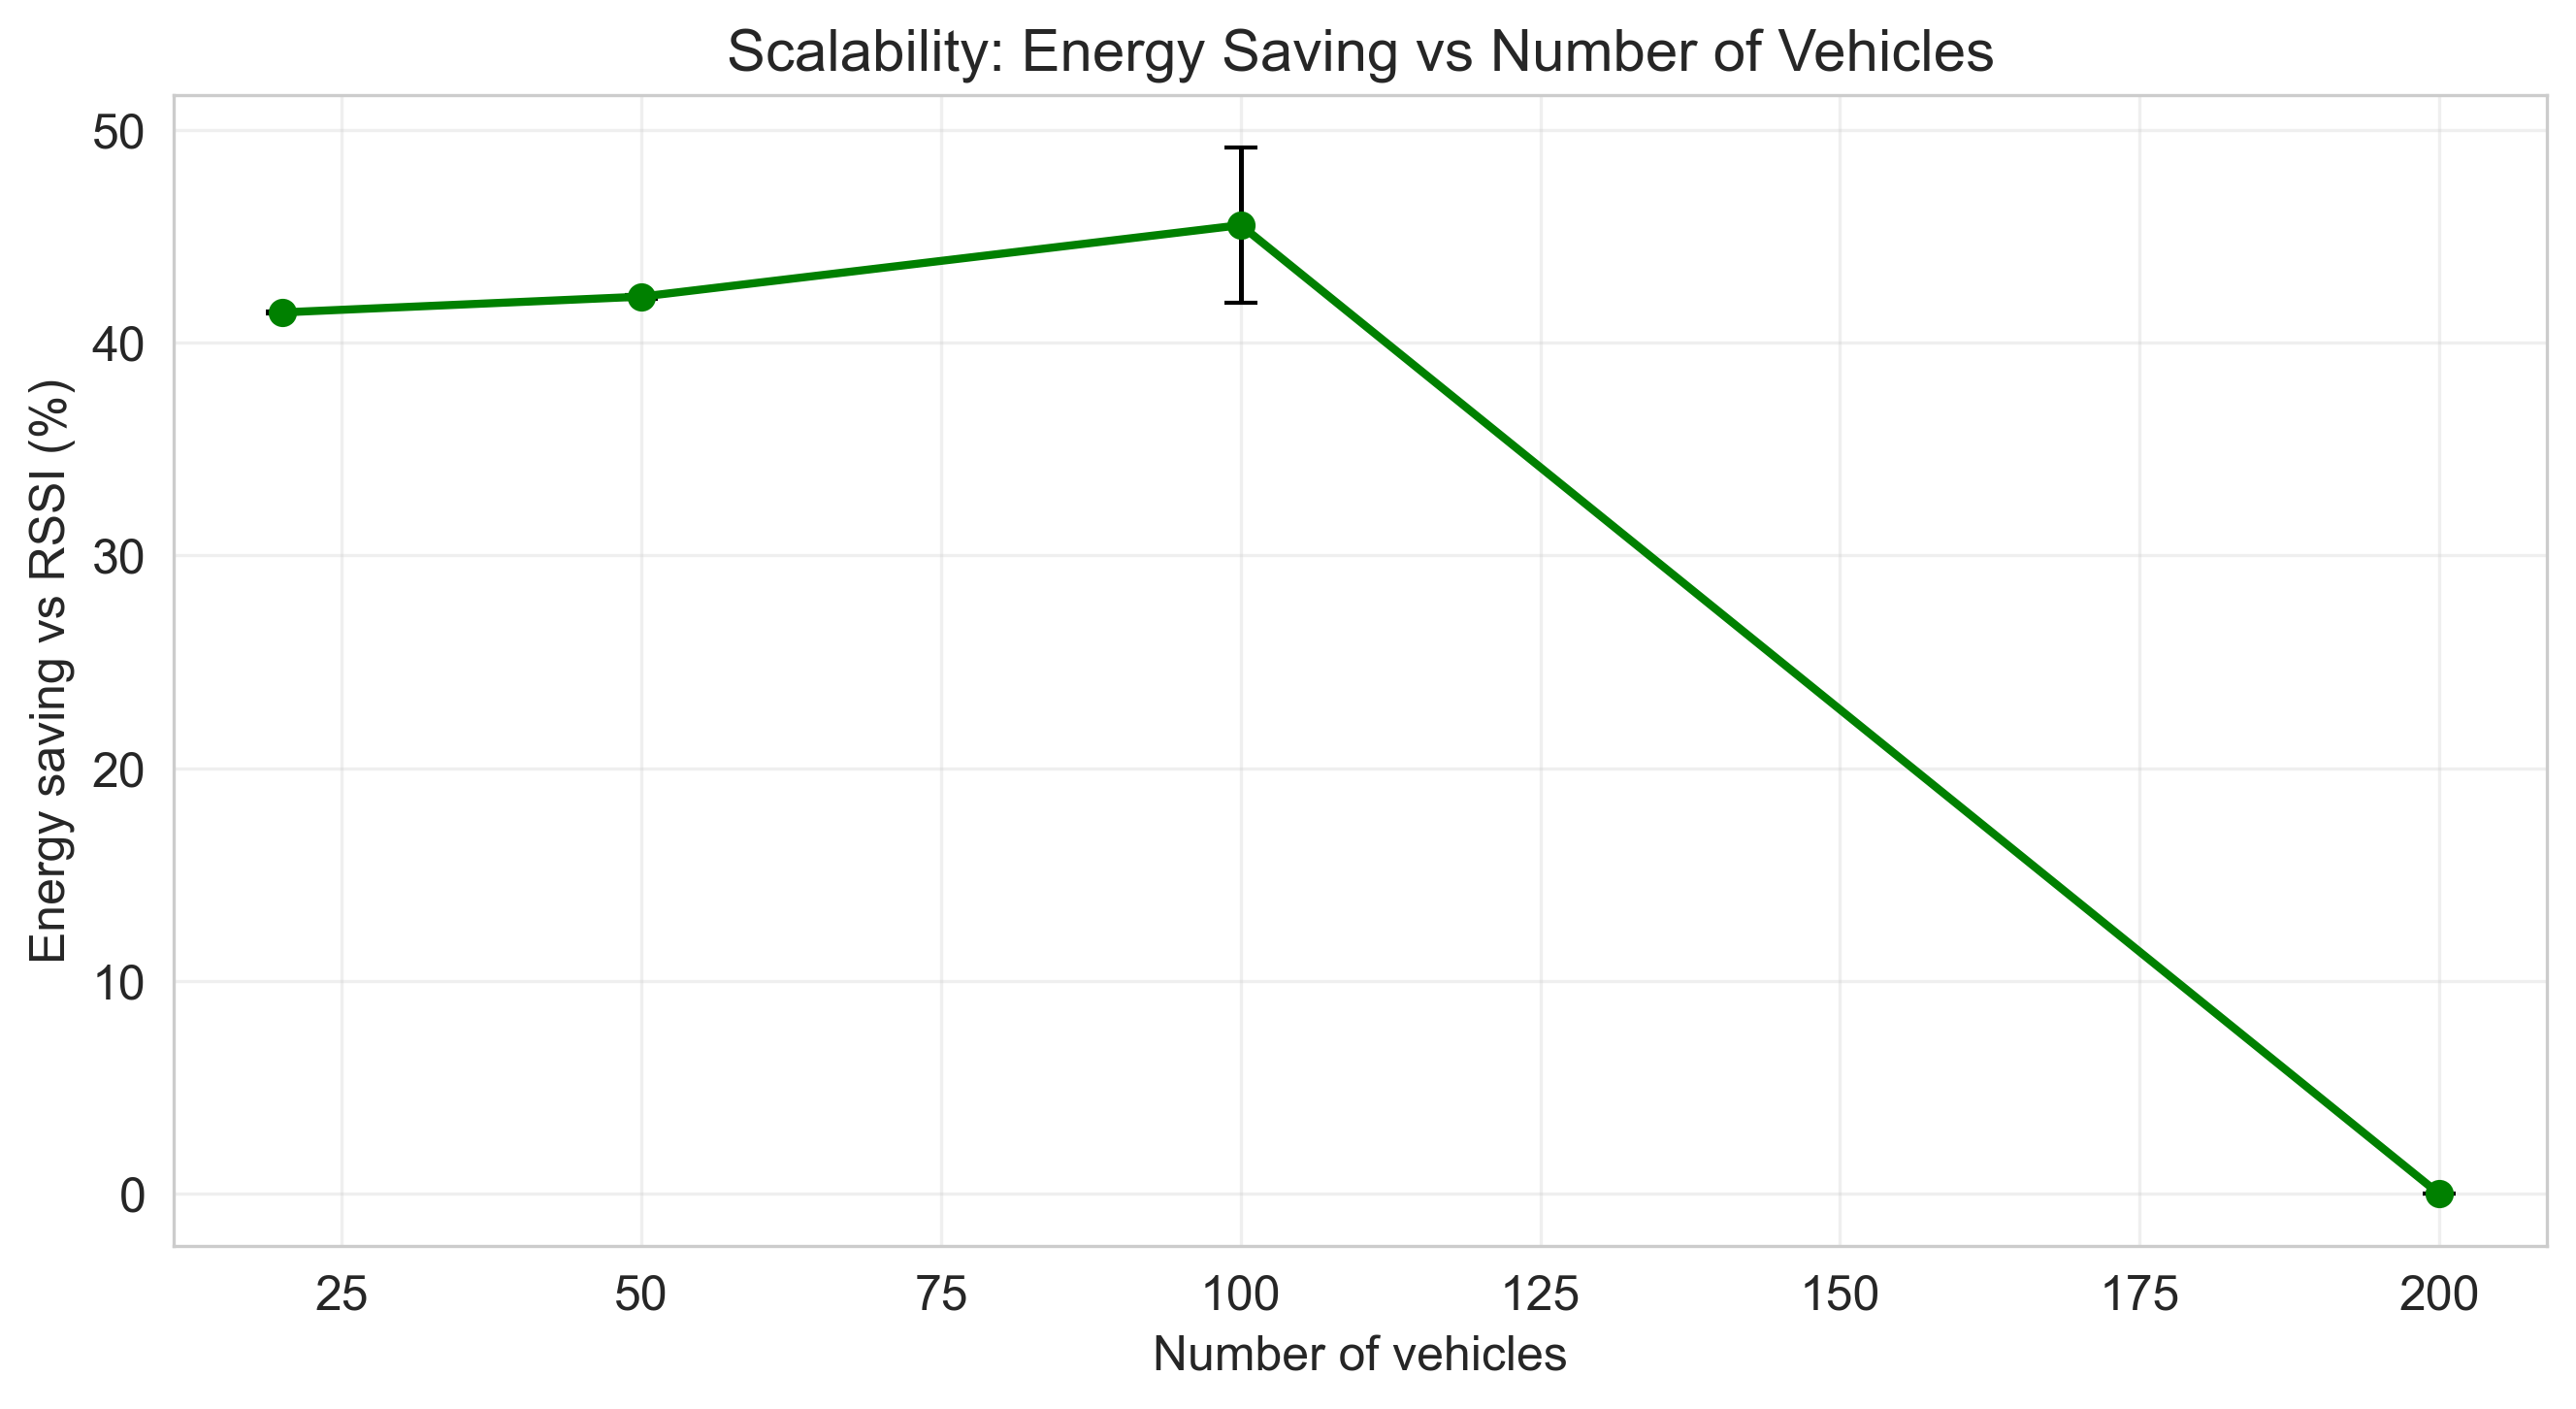
\includegraphics[width=\columnwidth]{results/scaling_energy_saving_vs_vehicles.png}
\caption{Scalability experiment: energy-saving trend versus number of vehicles.}
\label{fig:scaling_energy_saving_vs_vehicles}
\end{figure}


\subsection{3. Energy model validation \& sensitivity: \texttt{run_energy_model_sensitivity}}
\begin{itemize}
\item Vary two key parameters of \texttt{EnergyParams}:
\item \textbf{PA efficiency \texttt{eta\_pa}}:
\item Range: \texttt{[0.25, 0.35, 0.45]} (plausible PA efficiencies).
\item \textbf{TX circuit power \texttt{P\_tx\_circuit}}:
\item Range: \texttt{[0.05, 0.10, 0.15]} W.
\item For each value in each sweep:
\item Clone config with new seed from \texttt{SENSITIVITY\_SEEDS = [42, 123]}.
\item Create \texttt{V2XSimulator}.
\item Modify \texttt{sim.energy\_model.params} accordingly.
\item Also sync those parameters into \texttt{sim.energy\_aware\_algo.energy\_model.params}.
\item Run \texttt{run\_comparison()}.
\item Record \texttt{energy\_saving\_percent} vs RSSI.
\item Plot:
\item \texttt{energy\_model\_sensitivity.png}:
\item Left panel: saving vs \texttt{eta\_pa}.
\item Right panel: saving vs \texttt{P\_tx\_circuit}.
\item Save:
\item \texttt{energy\_model\_sensitivity.json} with sweep data.
\item \texttt{energy\_model\_justification.md} describing energy model and rationale.
\end{itemize}

\paragraph*{Goal}
\begin{itemize}
\item Show \textbf{EA advantage is robust} to plausible range of physical layer energy parameters.
\end{itemize}

\begin{figure}[t]
\centering
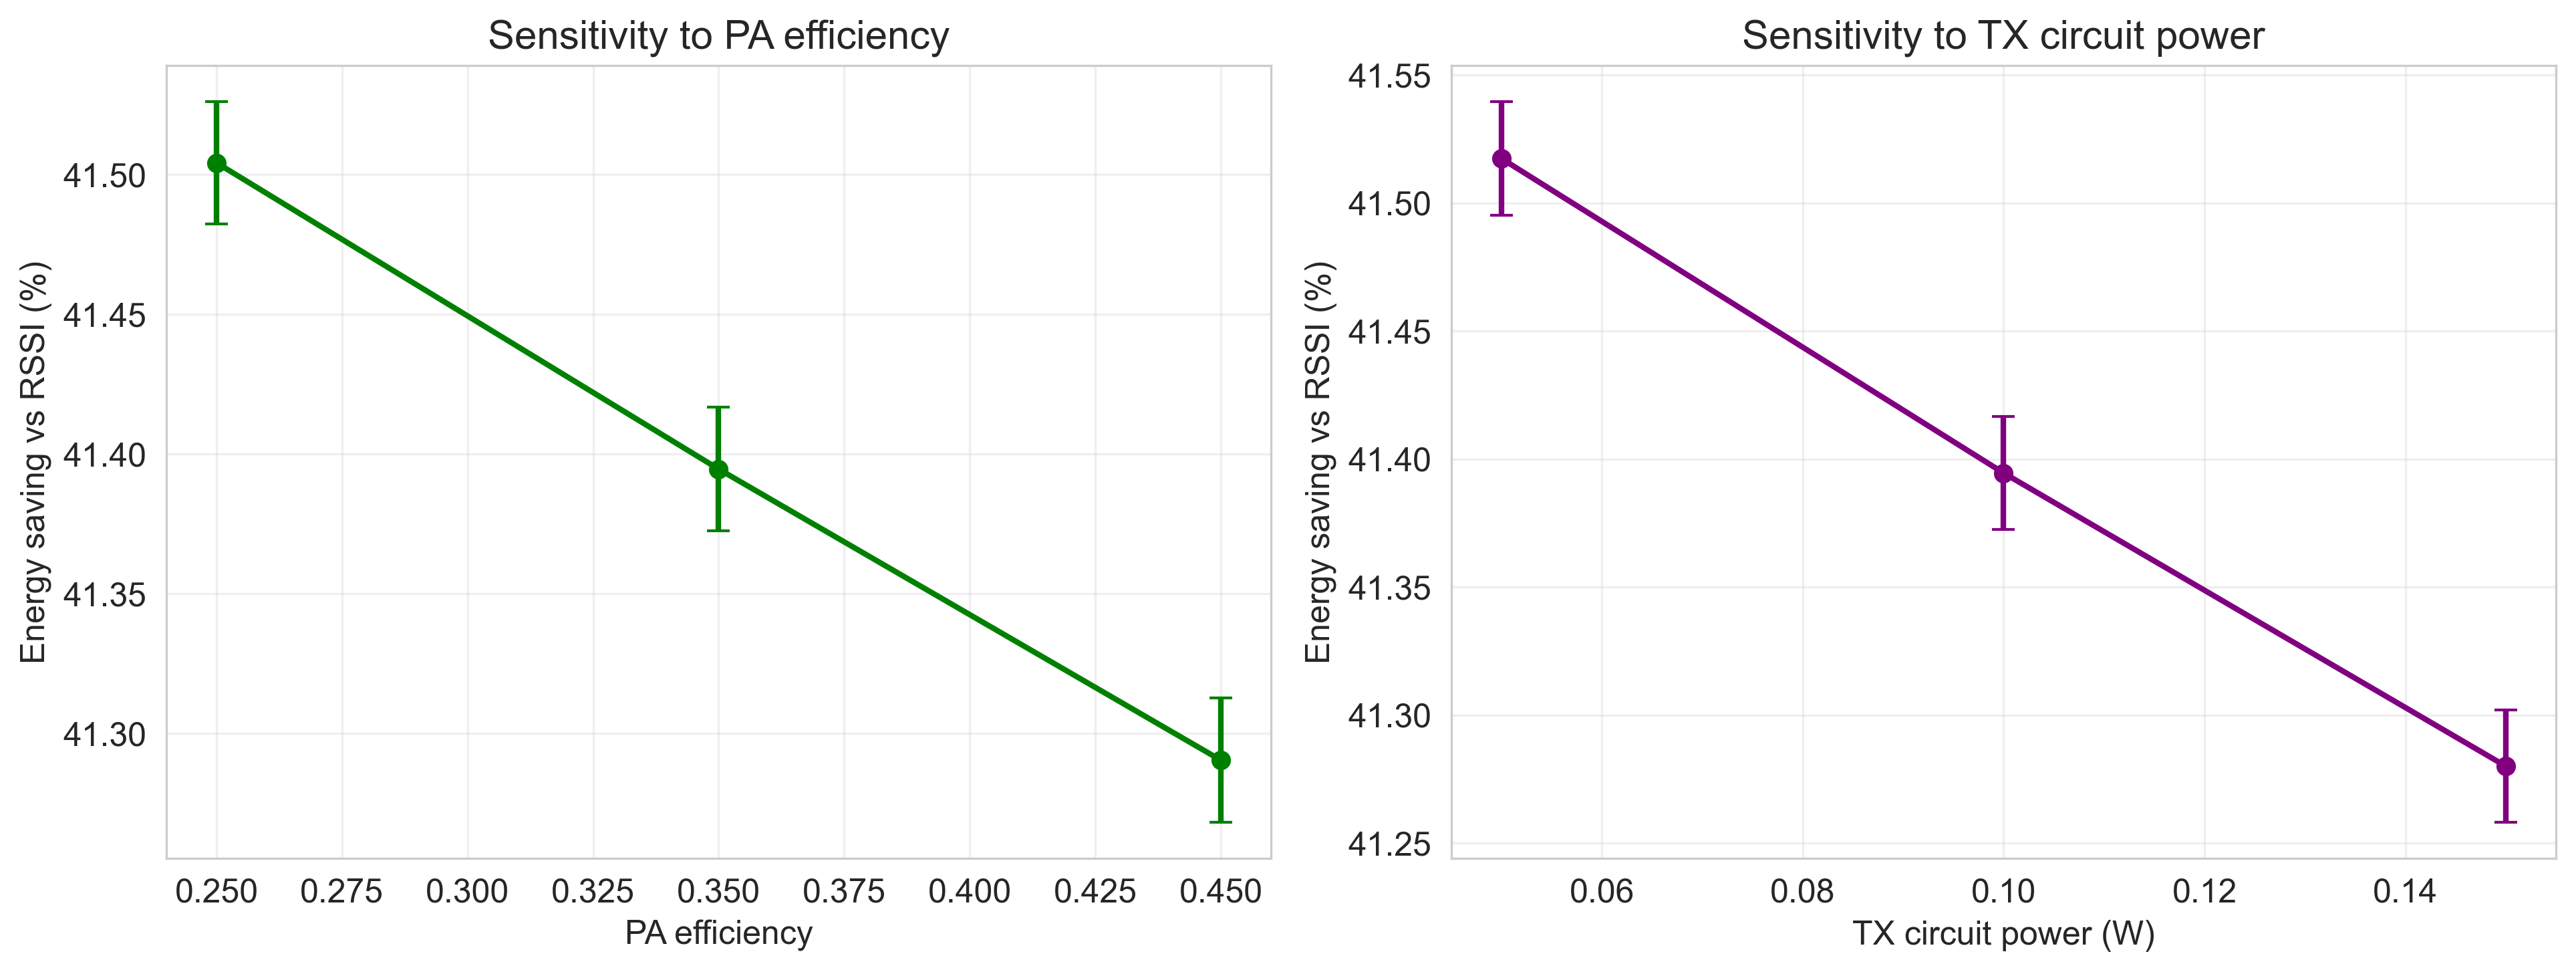
\includegraphics[width=\columnwidth]{results/energy_model_sensitivity.png}
\caption{Sensitivity of energy savings to PA efficiency and circuit power settings.}
\label{fig:energy_model_sensitivity}
\end{figure}


\subsection{4. Scenario diversity: \texttt{run_scenario_diversity_experiment}}
\begin{itemize}
\item Define three scenarios:
\item \textbf{Clear weather}:
\item \texttt{weather\_profile="clear"},
\item \texttt{shadowing\_std\_db=6},
\item \texttt{num\_base\_stations=9}, \texttt{area\_size}=base, \texttt{bs\_coverage\_radius}=base.
\item \textbf{Heavy rain}:
\item \texttt{weather\_profile="heavy\_rain"},
\item \texttt{shadowing\_std\_db=15},
\item \texttt{num\_base\_stations=9}.
\item \textbf{Urban dense}:
\item \texttt{weather\_profile="clear"},
\item \texttt{shadowing\_std\_db=18},
\item \texttt{num\_base\_stations=16},
\item \texttt{area\_size=2200}, \texttt{bs\_coverage\_radius=220}.
\item For each scenario and seeds \texttt{[42, 123, 456]}:
\item Clone config + apply overrides.
\item Run \texttt{run\_comparison()}.
\item Record \texttt{energy\_saving\_percent}.
\item Plot:
\item \texttt{scenario\_diversity\_energy\_saving.png}:
\item Bars (with error bars) for each scenario.
\item Save:
\item \texttt{scenario\_diversity\_results.json}, including:
\item Scenario definitions,
\item Per-seed savings,
\item Claim: EA maintains positive saving in all tested scenarios.
\end{itemize}

\paragraph*{Goal}
\begin{itemize}
\item Demonstrate \textbf{robustness across propagation/climate/density conditions}.
\end{itemize}

\begin{figure}[t]
\centering
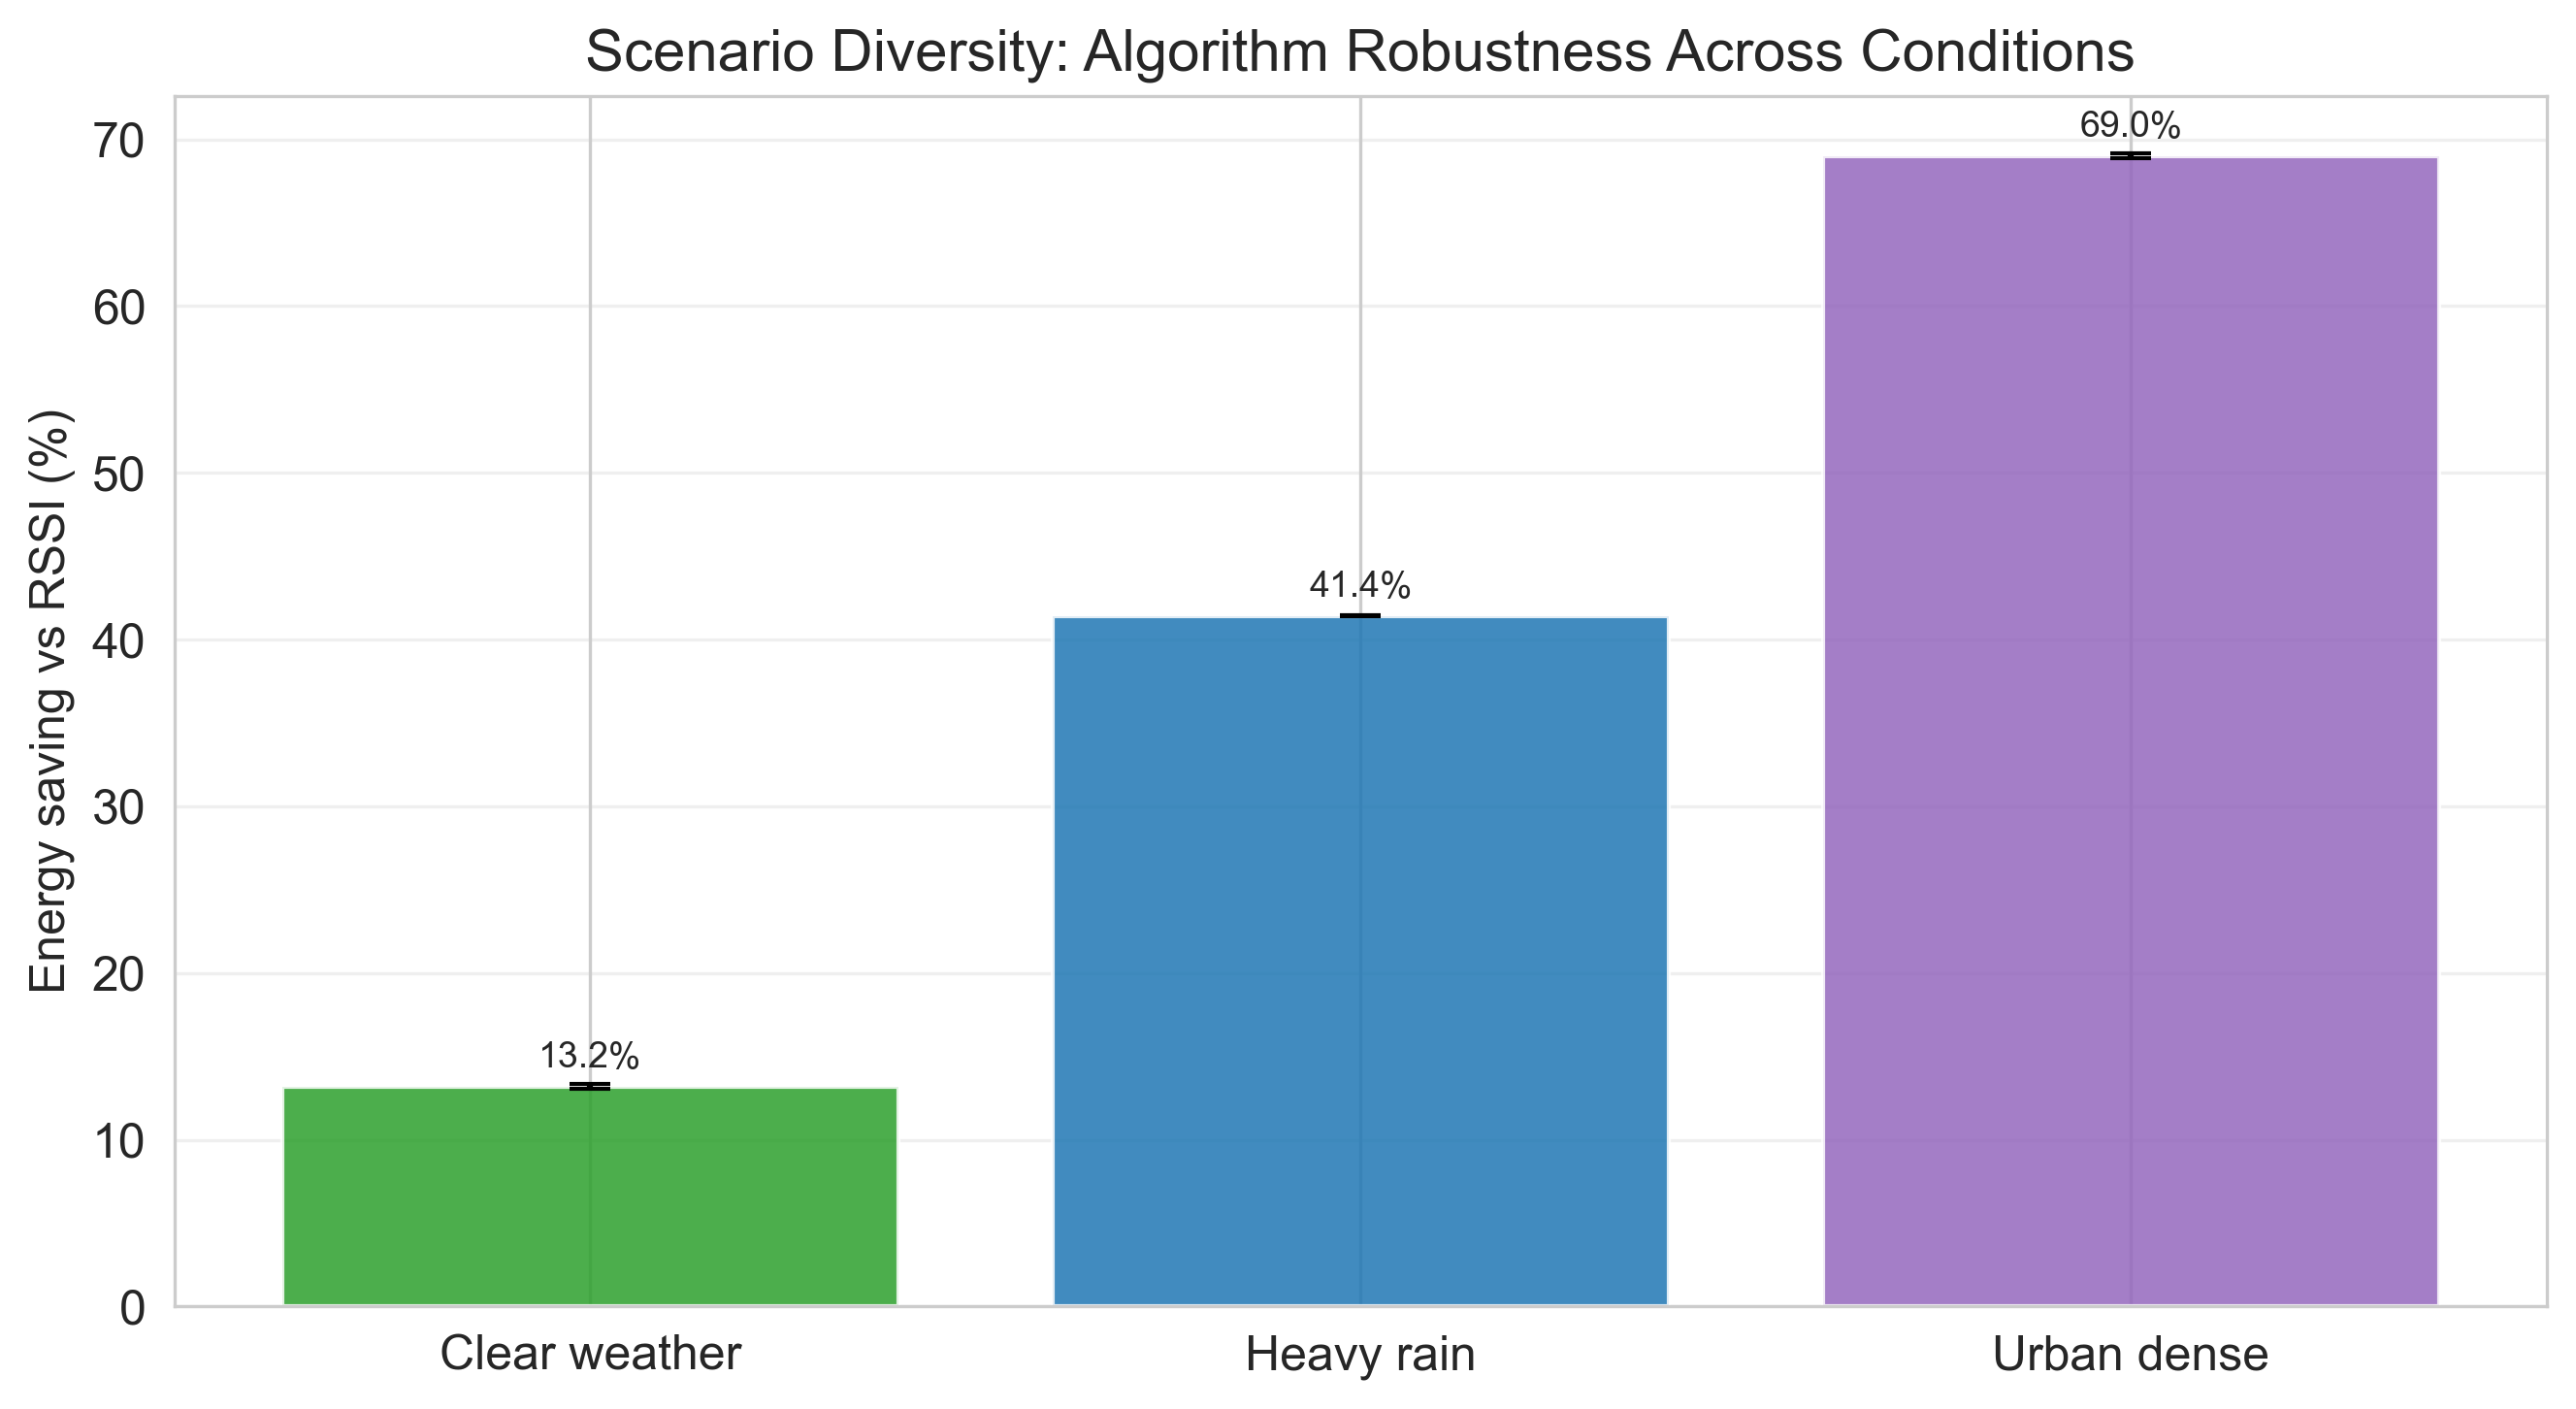
\includegraphics[width=\columnwidth]{results/scenario_diversity_energy_saving.png}
\caption{Scenario-diversity evaluation of energy savings across environments.}
\label{fig:scenario_diversity_energy_saving}
\end{figure}



\section{Tests: what they guarantee (\texttt{tests/test_simulation.py})}

The tests assert:
\begin{itemize}
\item \textbf{Environmental CO2 metrics are correct}:
\item 3.6e6 J at 0.5 kg/kWh → 0.5 kg CO2.
\item Derived per-vehicle metrics behave logically.
\item \textbf{Weather profiles}:
\item \texttt{SimulationConfig(weather\_profile="heavy\_rain")} returns correct path-loss and rain attenuation.
\item \textbf{Rain attenuation}:
\item Two BSs identical except \texttt{rain\_attenuation\_db\_per\_km}, difference in path loss at 1 km equals that attenuation.
\item \textbf{Shadowing percentile margin}:
\item Higher shadowing reliability (e.g., 0.95) → higher required TX power by \texttt{z * sigma} dB.
\item \textbf{Energy-aware QoS behavior}:
\item With moderate \texttt{min\_data\_rate\_bps}, algorithm chooses BS that meets QoS.
\item With extremely high \texttt{min\_data\_rate\_bps}, QoS not met, fallback is triggered (still returns some BS).
\item \textbf{Vehicle movement}:
\item Distance calculations,
\item Highway straight lanes and wrap behavior.
\item \textbf{BS coverage}:
\item Coverage disk membership works as expected.
\item \textbf{Simulator basic operation}:
\item Short run with small number of vehicles and BSs:
\item \texttt{run\_algorithm("rssi")} returns stats with all core fields present and in valid ranges.
\item \textbf{Stronger baselines}:
\item SINR and load-aware RSSI short runs produce valid stats.
\item \textbf{Link metrics}:
\item \texttt{\_make\_step\_link\_metrics\_getter} includes interference and SINR fields, which are non-negative and sensible.
\end{itemize}

These tests act like \textbf{unit + regression tests} to ensure that core modeling assumptions and metrics don’t silently break.


\section{Validation utilities and literature index (codebase)}

\begin{itemize}
\item \textbf{\texttt{src/utils/hardware\_validation.py}} --- \texttt{EnergyModelValidator}: compares representative model EPB to literature anchor rows; optional calibration factors for OBU/BS-style device types.
\item \textbf{\texttt{simulations/validator.py}} --- \texttt{ExtrapolationValidator}: runs multiple simulation durations and checks stability of per-second energy, CO\textsubscript{2}, and handoff rates (coefficient of variation); can save \texttt{results/extrapolation\_validation.png}.
\item \textbf{\texttt{simulations/config.py}} --- \texttt{extended\_validation\_scenario()}, \texttt{multi\_duration\_validation()}.
\item \textbf{\texttt{docs/literature\_review.py}} --- structured \texttt{LITERATURE\_REFERENCES} ($\approx$19 keys), \texttt{generate\_related\_work\_section()}, aligned with BibTeX keys for the final paper.
\item \textbf{\texttt{validation\_runner.py}} --- orchestrates comprehensive validation and optional JSON export (\texttt{results/comprehensive\_validation.json}).
\end{itemize}


\section{What is the aim of the project (in research terms)?}
\begin{itemize}
\item \textbf{Problem}: Classic handoff decisions (RSSI/SINR-based) do not explicitly consider \textbf{energy efficiency} or \textbf{CO2}; they might:
\item Overuse high-power links,
\item Overload some BSs while others are underused,
\item Cause unnecessary handoffs (ping-pong).
\item \textbf{Proposed idea}: A \textbf{handoff algorithm that minimizes energy per bit}, including a \textbf{load penalty}, while maintaining:
\item Good QoS (minimum data rate / SNR),
\item Limit on handoff churn (cooldown, time-to-trigger, ping-pong control).
\item \textbf{Evidence the project builds}:
\item Across:
\item Multiple seeds,
\item Different \textbf{vehicle counts},
\item Different \textbf{energy-model parameters},
\item Different \textbf{scenarios} (clear, heavy rain, urban dense),
\item The energy-aware algorithm:
\item Achieves \textbf{significant energy and CO2 savings} vs RSSI/SINR/load-aware RSSI and naive.
\item Maintains:
\item Similar or slightly improved \textbf{throughput},
\item Similar or improved \textbf{outage probability},
\item \textbf{No worse} handoff count than RSSI (often fewer),
\item Comparable or better \textbf{service availability}.
\end{itemize}

This positions the project as a \textbf{research-grade simulator} to back a \textbf{paper-style conclusion} about energy-aware handoff in V2X.



\section{Where this project excels (strengths)}
\begin{itemize}
\item \textbf{Rich modeling with reasonable complexity}:
\item Includes:
\item Mobility (highway / non-highway, lanes, lane speed differences).
\item Channel:
\item Path loss, shadowing,
\item Rain attenuation,
\item Interference and SINR.
\item Energy model:
\item PA efficiency,
\item RF circuits,
\item Baseband, cooling.
\item Environment:
\item Carbon intensity, operational CO\textsubscript{2}; optional extended scope in code; validation utilities.
\item \textbf{Multiple strong baselines}:
\item Not only naive vs new algorithm:
\item Includes RSSI, SINR, load-aware RSSI, naive nearest.
\item Baselines share same PHY model (adaptive TX for fairness).
\item \textbf{Robustness experiments}:
\item Scaling vs number of vehicles,
\item Sensitivity to physical energy model parameters,
\item Scenario diversity (weather, density).
\item \textbf{Detailed QoS \& stability metrics}:
\item Throughput (mean, p5),
\item Outage probability,
\item Service availability (mean, p5, std),
\item Outage burst statistics,
\item Handoff delay fraction,
\item Ping-pong rate.
\item \textbf{Good software structure}:
\item Separation into:
\item Config (\texttt{SimulationConfig}),
\item Models (\texttt{Vehicle}, \texttt{BaseStation}, \texttt{EnergyModel}),
\item Algorithms (5 strategies),
\item Simulator core,
\item Visualization utils,
\item Tests for critical parts.
\item \textbf{Reproducibility}:
\item Seeds are controlled and rerun for each algorithm.
\item Results saved as JSON with config embedded, plus plots.
\end{itemize}



\section{Limitations / assumptions (where it does NOT model everything)}

Understanding limits is as important as strengths:
\begin{itemize}
\item \textbf{Traffic model}:
\item Data rate is “offered” via a Shannon formula tied to SINR; no explicit packet arrivals, queueing delays, or application traffic patterns.
\item \textbf{MAC / scheduling}:
\item Load is a scalar \texttt{load} per BS; the actual per-user scheduling policy is abstracted.
\item No explicit modeling of time-slot allocation, HARQ, or retransmissions (only captured via SINR/outage logic).
\item \textbf{Interference modeling}:
\item All BSs assumed to transmit into the same bandwidth with target RX, so interference is approximated by each BS’s own link budget to the vehicle, not full LTE/NR scheduler.
\item \textbf{Mobility simplifications}:
\item Highway lanes are straight with wrap boundaries.
\item No intersections, no traffic rules (stopping, acceleration, braking), collisions, etc.
\item \textbf{Energy model}:
\item Focused on RF chain + baseband + cooling.
\item Does not explicitly model:
\item Control plane signaling overhead,
\item BS sleep modes (beyond simple sleep/idle states),
\item Vehicle ECU or sensor energy.
\item \textbf{Scalability}:
\item Simulations can be CPU-intensive for very large numbers of vehicles / BSs because each step evaluates links to multiple BSs.
\item \textbf{CO\textsubscript{2} and annual figures}:
\item Stated \textbf{scope}: operational communication energy and grid CO\textsubscript{2} proxy only; not propulsion, manufacturing, or backhaul (see dedicated section above).
\item \textbf{Yearly CO\textsubscript{2}} from short simulations is a \textbf{linear extrapolation}; for absolute annual claims, apply a \textbf{duty cycle} or label as worst-case continuous operation.
\item \textbf{Grid intensity}: default 0.5~kg/kWh is illustrative; regional factors (e.g.\ Bangladesh $\approx$0.6--0.65~kg/kWh) require citation to national/grid sources when reported.
\item \textbf{Hardware validation}: literature EPB anchors are sanity checks, not substitute for measured traces from a physical testbed.
\end{itemize}

These are reasonable simplifications for a \textbf{handoff \& energy} study, but you should be aware if you extend it toward, say, full 3GPP-grade system-level simulations.



\section{How to mentally walk through “what happens when I run \texttt{python main.py}”}
\begin{itemize}
\item \textbf{Config \& logging}:
\item Build a demonstration \texttt{SimulationConfig}.
\item Print scenario settings (vehicles, BSs, duration, area, shadowing, weather, carbon intensity, seeds, etc.).
\item \textbf{For each seed}:
\item Set \texttt{config.seed}.
\item Build \texttt{V2XSimulator(config)}.
\item Run:
\item \texttt{setup\_network} → grid of BSs under chosen weather.
\item \texttt{setup\_vehicles} → initial vehicle placements/speeds.
\item \texttt{run\_comparison}:
\item For each algorithm:
\item Reset vehicles and random seed.
\item Run time loop:
\item Move vehicles, maybe change lanes.
\item Compute link metrics, decide handoffs.
\item Accumulate energy, bits, outages, etc.
\item Compute cross-algorithm improvements (energy saving, CO2, handoffs).
\item Append per-seed comparison into list.
\item \textbf{After all seeds}:
\item Compute multiple \textbf{mean ± std} stats.
\item Run \textbf{paired t-tests} (RSSI vs EA).
\item Compute aggregated CO2 metrics.
\item \textbf{Output \& plots}:
\item Save last simulator result as JSON.
\item Use \texttt{ResultVisualizer} to produce:
\item Energy comparison, cumulative CO2, per-vehicle CDF, bar charts, distributions, topology.
\item \textbf{Extra experiments}:
\item Run scalability (vary num vehicles).
\item Run energy-model sensitivity sweeps.
\item Run scenario diversity.
\item \textbf{Final console summary}:
\item Print detailed per-algorithm stats for last seed.
\item Print improvements (savings vs baselines).
\item Provide mechanistic explanation:
\item Differences in TX power distributions,
\item BS load distribution,
\item SINR histogram.
\end{itemize}



\section{If you want, next steps I can walk through}

If you’d like even deeper detail, I can:
\begin{itemize}
\item Break down \textbf{each algorithm’s source code} line-by-line (e.g., \texttt{energy\_aware\_handoff.py}).
\item Derive the \textbf{exact formula} for \texttt{calculate\_tx\_power\_required\_for\_target\_rx} and show how shadowing percentile enters.
\item Show \textbf{concrete example numbers} for a single vehicle over a few steps to see energy and handoffs.
\item Help you \textbf{modify the scenario} (e.g., urban highway, longer duration) and interpret new plots.
\end{itemize}

\paragraph*{1) Line-by-line algorithm walkthrough}
The most useful deep-dive starts from a common interface view and then compares decision logic block by block. In practice, I can walk through \texttt{select\_best\_bs(...)}, \texttt{should\_handoff(...)}, and \texttt{execute\_handoff(...)} for Energy-Aware, RSSI, SINR, load-aware RSSI, and naive-nearest policies side by side. The review can explicitly map each code branch to its system objective: energy minimization, signal-quality maximization, load balancing, and stability protection. I can also annotate which lines are model assumptions versus implementation safeguards (e.g., capacity checks, fallback behavior, cooldown checks, and ping-pong accounting), so your methods section can cite behavior unambiguously.

\paragraph*{2) Exact TX-power and shadowing derivation}
I can provide a full derivation from link-budget fundamentals to the implemented function \texttt{calculate\_tx\_power\_required\_for\_target\_rx}. This includes: distance-dependent path loss, rain attenuation, log-normal shadowing margin, receiver target power, and conversion between dBm and linear watts. A key part is the reliability margin: when coverage is designed for a percentile (e.g., 95\%), the model effectively adds a positive margin proportional to shadowing standard deviation, which increases required transmit power. I can present the final closed-form expression used in code, explain each term physically, and show how changing weather profile parameters shifts required power and therefore energy-per-bit outcomes.

\paragraph*{3) Concrete numerical trajectory example}
For publication clarity, I can produce a worked micro-trace for one vehicle over several time steps: position, candidate BS metrics, selected BS, SINR, data rate, transmit power, per-step energy, and handoff trigger outcome. This makes the algorithm mechanics transparent and helps reviewers verify that performance gains are not black-box artifacts. The walkthrough can include one case where a handoff is blocked by hysteresis/cooldown and another where it is accepted due to sufficient EPB gain under QoS constraints. I can format this as a compact table-ready narrative you can directly adapt into the paper.

\paragraph*{4) Scenario redesign and plot interpretation support}
I can help you create targeted scenario variants (e.g., longer simulation duration, denser traffic, stronger shadowing, different weather, modified BS density, stricter outage threshold) and predict how each change should affect key metrics before running experiments. After execution, I can guide interpretation of each figure type: whether shifts are due to load balancing, power control, interference exposure, or mobility-induced instability. This is especially useful for writing discussion and threat-to-validity sections, where you need to explain not only ``what improved'' but also ``why it improved'' and ``under what conditions gains shrink.''


\begin{thebibliography}{00}

\bibitem{auer2011howmuch}
G.~Auer \emph{et al.}, ``How much energy is needed to run a wireless network?,'' \emph{IEEE Wireless Commun.}, vol.~18, no.~5, pp.~40--49, Oct. 2011.

\bibitem{hasan2011green}
Z.~Hasan, H.~Boostanimehr, and V.~K.~Bhargava, ``Green cellular networks: A survey, some research issues and challenges,'' \emph{IEEE Commun. Surveys Tuts.}, vol.~13, no.~4, pp.~524--540, Fourth Quarter 2011.

\bibitem{chen2011fundamental}
T.~Chen, H.~Kim, and Y.~Yang, ``Fundamental trade-offs on green wireless networks,'' \emph{IEEE Commun. Mag.}, vol.~49, no.~6, pp.~30--37, Jun. 2011.

\bibitem{malmodin2018global}
J.~Malmodin and D.~Lund\'{e}n, ``The energy and carbon footprint of the global ICT and E\&M sectors 2010--2015,'' \emph{Sustainability}, vol.~10, no.~9, 2018.

\bibitem{abboud2016interworking}
K.~Abboud, H.~A.~Omar, and W.~Zhuang, ``Interworking of DSRC and cellular network technologies for V2X communications: A survey,'' \emph{IEEE Trans. Veh. Technol.}, vol.~65, no.~12, pp.~9457--9474, Dec. 2016.

\end{thebibliography}

\end{document}
